%% abtex2-modelo-trabalho-academico.tex, v-1.9.7 laurocesar
%% Copyright 2012-2018 by abnTeX2 group at http://www.abntex.net.br/ 
%%
%% This work may be distributed and/or modified under the
%% conditions of the LaTeX Project Public License, either version 1.3
%% of this license or (at your option) any later version.
%% The latest version of this license is in
%%   http://www.latex-project.org/lppl.txt
%% and version 1.3 or later is part of all distributions of LaTeX
%% version 2005/12/01 or later.
%%
%% This work has the LPPL maintenance status `maintained'.
%% 
%% The Current Maintainer of this work is the abnTeX2 team, led
%% by Lauro César Araujo. Further information are available on 
%% http://www.abntex.net.br/
%%
%% This work consists of the files abntex2-modelo-trabalho-academico.tex,
%% abntex2-modelo-include-comandos and abntex2-modelo-references.bib
%%

% ------------------------------------------------------------------------
% ------------------------------------------------------------------------
% abnTeX2: Modelo de Trabalho Academico (tese de doutorado, dissertacao de
% mestrado e trabalhos monograficos em geral) em conformidade com 
% ABNT NBR 14724:2011: Informacao e documentacao - Trabalhos academicos -
% Apresentacao
% ------------------------------------------------------------------------
% ------------------------------------------------------------------------

\documentclass[
	% -- opções da classe memoir --
	12pt,				% tamanho da fonte
	openany,			% capítulos começam em pág ímpar (insere página vazia caso preciso)
	twoside,			% para impressão em recto e verso. Oposto a oneside
	a4paper,			% tamanho do papel. 
	% -- opções da classe abntex2 --
	%chapter=TITLE,		% títulos de capítulos convertidos em letras maiúsculas
	%section=TITLE,		% títulos de seções convertidos em letras maiúsculas
	%subsection=TITLE,	% títulos de subseções convertidos em letras maiúsculas
	%subsubsection=TITLE,% títulos de subsubseções convertidos em letras maiúsculas
	% -- opções do pacote babel --
	english,			% idioma adicional para hifenização
	french,				% idioma adicional para hifenização
	spanish,			% idioma adicional para hifenização
	brazil				% o último idioma é o principal do documento
	]{abntex2}

\checkandfixthelayout % para garantir que o layout seja atualizado
\makeatletter
\renewcommand*{\cleardoublepage}{\clearpage}
\makeatother
% ---
% Pacotes básicos 
% ---
\usepackage{emptypage}
\usepackage{longtable}
\usepackage{float}
\usepackage{lmodern}			% Usa a fonte Latin Modern			
\usepackage[T1]{fontenc}		% Selecao de codigos de fonte.
\usepackage[utf8]{inputenc}		% Codificacao do documento (conversão automática dos acentos)
\usepackage{indentfirst}		% Indenta o primeiro parágrafo de cada seção.
\usepackage{color}				% Controle das cores
\usepackage{graphicx}			% Inclusão de gráficos
\usepackage{microtype} 			% para melhorias de justificação
% ---
		
% ---
% Pacotes adicionais, usados apenas no âmbito do Modelo Canônico do abnteX2
% ---
\usepackage{pgfplots}
\pgfplotsset{compat=1.18}
\usepackage{adjustbox}
\usepackage{ragged2e}
\usepackage{tabularx}
\usepackage{array}
\usepackage{booktabs} % para tabelas com linhas bonitas
\usepackage[utf8]{inputenc}
\usepackage{geometry}
\geometry{margin=1in}
\usepackage{lipsum}				% para geração de dummy text
% ---

% ---
% Pacotes de citações
% ---
\usepackage[brazilian,hyperpageref]{backref}	 % Paginas com as citações na bibl
\usepackage[alf]{abntex2cite}	% Citações padrão ABNT

% --- 
% CONFIGURAÇÕES DE PACOTES
% --- 

% ---
% Configurações do pacote backref
% Usado sem a opção hyperpageref de backref
\renewcommand{\backrefpagesname}{Citado na(s) página(s):~}
% Texto padrão antes do número das páginas
\renewcommand{\backref}{}
% Define os textos da citação
\renewcommand*{\backrefalt}[4]{
	\ifcase #1 %
		Nenhuma citação no texto.%
	\or
		Citado na página #2.%
	\else
		Citado #1 vezes nas páginas #2.%
	\fi}%
% ---

% ---
% Informações de dados para CAPA e FOLHA DE ROSTO
% ---
\titulo{Pousada Chalés Água de Coco}
\autor{ANNA JULIA LIMA DE SOUSA SP3024016\\ GUILHERME AKIO MIURA SP3120791\\ GUILHERME BITTENCOURT SCHMIDT SP313640X\\KELLY RADCHELLE ARAUJO DE SOUZA SP3123588\\RAFAEL TEIXEIRA FONSECA SP3126919\\ RICARDO CARRIEL DE OLIVEIRA FILHO SP3136728}
\local{São Paulo - SP - Brasil}
\data{2025}
\orientador{Marcelo Tavares de Santana}
%\coorientador{Equipe \abnTeX}
\instituicao{%
  IFSP - Instituto Federal de Educação, Ciência e Tecnologia de São Paulo
  \par
  Tecnologia em Análise e Desenvolvimento de Sistemas}
\tipotrabalho{Trabalho Conclusão de Curso}
% O preambulo deve conter o tipo do trabalho, o objetivo, 
% o nome da instituição e a área de concentração 
\preambulo{Trabalho de Conclusão de Curso apresentado
ao Instituto Federal de Educação, Ciência e
Tecnologia de São Paulo Câmpus São Paulo,
como requisito parcial para conclusão do
curso Tecnologia em Análise e Desenvolvimento de Sistemas \LaTeX.}
% ---


% ---
% Configurações de aparência do PDF final

% alterando o aspecto da cor azul
\definecolor{blue}{RGB}{41,5,195}

% informações do PDF
\makeatletter
\hypersetup{
     	%pagebackref=true,
		pdftitle={\@title}, 
		pdfauthor={\@author},
    	pdfsubject={\imprimirpreambulo},
	    pdfcreator={LaTeX with abnTeX2},
		pdfkeywords={abnt}{latex}{abntex}{abntex2}{trabalho acadêmico}, 
		colorlinks=true,       		% false: boxed links; true: colored links
    	linkcolor=blue,          	% color of internal links
    	citecolor=blue,        		% color of links to bibliography
    	filecolor=magenta,      		% color of file links
		urlcolor=blue,
		bookmarksdepth=4
}
\makeatother
% --- 

% ---
% Posiciona figuras e tabelas no topo da página quando adicionadas sozinhas
% em um página em branco. Ver https://github.com/abntex/abntex2/issues/170
\makeatletter
\setlength{\@fptop}{5pt} % Set distance from top of page to first float
\makeatother
% ---

% ---
% Possibilita criação de Quadros e Lista de quadros.
% Ver https://github.com/abntex/abntex2/issues/176
%
\newcommand{\quadroname}{Quadro}
\newcommand{\listofquadrosname}{Lista de quadros}

\floatstyle{plain}
\newfloat{quadro}{htbp}{loq}
\floatname{quadro}{Quadro}
%\newfloat[chapter]{quadro}{loq}{\quadroname}
\newlistof{listofquadros}{loq}{\listofquadrosname}
\newlistentry{quadro}{loq}{0}

% configurações para atender às regras da ABNT
\setfloatadjustment{quadro}{\centering}
\counterwithout{quadro}{chapter}
\renewcommand{\cftquadroname}{\quadroname\space} 
\renewcommand*{\cftquadroaftersnum}{\hfill--\hfill}

\setfloatlocations{quadro}{hbtp} % Ver https://github.com/abntex/abntex2/issues/176
% ---

% --- 
% Espaçamentos entre linhas e parágrafos 
% --- 

% O tamanho do parágrafo é dado por:
\setlength{\parindent}{1.3cm}

% Controle do espaçamento entre um parágrafo e outro:
\setlength{\parskip}{0.2cm}  % tente também \onelineskip

% ---
% compila o indice
% ---
\makeindex
% ---

% ----
% Início do documento
% ----
\begin{document}

% Seleciona o idioma do documento (conforme pacotes do babel)
%\selectlanguage{english}
\selectlanguage{brazil}

% Retira espaço extra obsoleto entre as frases.
\frenchspacing 

% ----------------------------------------------------------
% ELEMENTOS PRÉ-TEXTUAIS
% ----------------------------------------------------------
% \pretextual

% ---
% Capa
% ---
\imprimircapa
% ---
% ---
% Folha de rosto
% (o * indica que haverá a ficha bibliográfica)
% ---
\imprimirfolhaderosto*
% ---
% ---
% Inserir a ficha bibliografica
% ---
% Isto é um exemplo de Ficha Catalográfica, ou ``Dados internacionais de
% catalogação-na-publicação''. Você pode utilizar este modelo como referência. 
% Porém, provavelmente a biblioteca da sua universidade lhe fornecerá um PDF
% com a ficha catalográfica definitiva após a defesa do trabalho. Quando estiver
% com o documento, salve-o como PDF no diretório do seu projeto e substitua todo
% o conteúdo de implementação deste arquivo pelo comando abaixo:
%
% \begin{fichacatalografica}
%     \includepdf{fig_ficha_catalografica.pdf}
% \end{fichacatalografica}
%\begin{fichacatalografica}
%	\sffamily
%	\vspace*{\fill}					% Posição vertical
%	\begin{center}					% Minipage Centralizado
%	\fbox{\begin{minipage}[c][8cm]{13.5cm}		% Largura
%	\small
%	\imprimirautor
	%Sobrenome, Nome do autor
	
%	\hspace{0.5cm} \imprimirtitulo  / \imprimirautor. --
%	\imprimirlocal, \imprimirdata-
	
%	\hspace{0.5cm} \thelastpage p. : il. (algumas color.) ; 30 cm.\\
	
%	\hspace{0.5cm} \imprimirorientadorRotulo~\imprimirorientador\\
	
%	\hspace{0.5cm}
%	\parbox[t]{\textwidth}{\imprimirtipotrabalho~--~\imprimirinstituicao,
%	\imprimirdata.}\\
	
%	\hspace{0.5cm}
%		1. Palavra-chave1.
%		2. Palavra-chave2.
%		2. Palavra-chave3.
%		I. Orientador.
%		II. Universidade xxx.
%		III. Faculdade de xxx.
%		IV. Título 			
%	\end{minipage}}
%	\end{center}
%\end{fichacatalografica}
% ---

% ---
% Inserir errata
% ---
%\begin{errata}
%Elemento opcional da \citeonline[4.2.1.2]{NBR14724:2011}. Exemplo:

%\vspace{\onelineskip}

%FERRIGNO, C. R. A. \textbf{Tratamento de neoplasias ósseas apendiculares com
%reimplantação de enxerto ósseo autólogo autoclavado associado ao plasma
%rico em plaquetas}: estudo crítico na cirurgia de preservação de membro em
%cães. 2011. 128 f. Tese (Livre-Docência) - Faculdade de Medicina Veterinária e
%Zootecnia, Universidade de São Paulo, São Paulo, 2011.

%\begin{table}[htb]
%\center
%\footnotesize
%\begin{tabular}{|p{1.4cm}|p{1cm}|p{3cm}|p{3cm}|}
%  \hline
%   \textbf{Folha} & \textbf{Linha}  & \textbf{Onde se lê}  & \textbf{Leia-se}  \\
%    \hline
%    1 & 10 & auto-conclavo & autoconclavo\\
%   \hline
%\end{tabular}
%\end{table}

%\end{errata}
% ---

% ---
% Inserir folha de aprovação
% ---

% Isto é um exemplo de Folha de aprovação, elemento obrigatório da NBR
% 14724/2011 (seção 4.2.1.3). Você pode utilizar este modelo até a aprovação
% do trabalho. Após isso, substitua todo o conteúdo deste arquivo por uma
% imagem da página assinada pela banca com o comando abaixo:
%
% \begin{folhadeaprovacao}
% \includepdf{folhadeaprovacao_final.pdf}
% \end{folhadeaprovacao}
%
%\begin{folhadeaprovacao}

%  \begin{center}
%    {\ABNTEXchapterfont\large\imprimirautor}

%    \vspace*{\fill}\vspace*{\fill}
%    \begin{center}
%      \ABNTEXchapterfont\bfseries\Large\imprimirtitulo
%    \end{center}
%    \vspace*{\fill}
    
%    \hspace{.45\textwidth}
%    \begin{minipage}{.5\textwidth}
 %       \imprimirpreambulo
%    \end{minipage}%
%    \vspace*{\fill}
%   \end{center}
        
%   Trabalho aprovado. \imprimirlocal, 24 de novembro de 2012:

%   \assinatura{\textbf{\imprimirorientador} \\ Orientador} 
%   \assinatura{\textbf{Professor} \\ Convidado 1}
%   \assinatura{\textbf{Professor} \\ Convidado 2}
   %\assinatura{\textbf{Professor} \\ Convidado 3}
   %\assinatura{\textbf{Professor} \\ Convidado 4}
      
%   \begin{center}
%    \vspace*{0.5cm}
%    {\large\imprimirlocal}
%    \par
%    {\large\imprimirdata}
%    \vspace*{1cm}
%  \end{center}
  
%\end{folhadeaprovacao}
% ---

% ---
% Dedicatória
% ---
%\begin{dedicatoria}
%   \vspace*{\fill}
%   \centering
%   \noindent
%   \textit{ Este trabalho é dedicado às crianças adultas que,\\
%   quando pequenas, sonharam em se tornar cientistas.} \vspace*{\fill}
%\end{dedicatoria}
% ---

% ---
% Agradecimentos
% ---
%\begin{agradecimentos}
%Os agradecimentos principais são direcionados à Gerald Weber, Miguel Frasson,
%Leslie H. Watter, Bruno Parente Lima, Flávio de Vasconcellos Corrêa, Otavio Real
%Salvador, Renato Machnievscz\footnote{Os nomes dos integrantes do primeiro
%projeto abn\TeX\ foram extraídos de
%\url{http://codigolivre.org.br/projects/abntex/}} e todos aqueles que
%contribuíram para que a produção de trabalhos acadêmicos conforme
%as normas ABNT com \LaTeX\ fosse possível.

%Agradecimentos especiais são direcionados ao Centro de Pesquisa em Arquitetura
%da Informação\footnote{\url{http://www.cpai.unb.br/}} da Universidade de
%Brasília (CPAI), ao grupo de usuários
%\emph{latex-br}\footnote{\url{http://groups.google.com/group/latex-br}} e aos
%novos voluntários do grupo
%\emph{\abnTeX}\footnote{\url{http://groups.google.com/group/abntex2} e
%\url{http://www.abntex.net.br/}}~que contribuíram e que ainda
%contribuirão para a evolução do \abnTeX.

%\end{agradecimentos}
% ---

% ---
% Epígrafe
% ---
%\begin{epigrafe}
%    \vspace*{\fill}
%	\begin{flushright}
%		\textit{``Não vos amoldeis às estruturas deste mundo, \\
%		mas transformai-vos pela renovação da mente, \\
%		a fim de distinguir qual é a vontade de Deus: \\
%		o que é bom, o que Lhe é agradável, o que é perfeito.\\
%		(Bíblia Sagrada, Romanos 12, 2)}
%	\end{flushright}
%\end{epigrafe}
% ---

% ---
% RESUMOS
% ---

% resumo em português
\setlength{\absparsep}{18pt} % ajusta o espaçamento dos parágrafos do resumo
\begin{resumo}
	Este Projeto de Conclusão de Curso tem como objetivo o desenvolvimento de um sistema web para automatizar os processos administrativos da pousada Chalés Água de Coco, que atualmente realiza a gestão de hóspedes, reservas, acomodações e controle financeiro por meio de planilhas eletrônicas no Excel. A falta de integração e a limitação desse método tornam a operação vulnerável a erros, retrabalho e dificuldade de acesso remoto às informações. Com base em uma parceria estabelecida com a pousada, foi possível realizar um levantamento detalhado dos requisitos e desenvolver uma solução personalizada, capaz de centralizar as informações em uma única plataforma, acessível via internet. O sistema propõe melhorias significativas na organização dos dados, no controle de reservas e na geração de relatórios gerenciais, otimizando a tomada de decisões. Este projeto representa a aplicação prática dos conhecimentos adquiridos ao longo do curso, ao mesmo tempo em que oferece uma ferramenta útil para a modernização da gestão em pequenos empreendimentos do setor de hospitalidade.
	
	\textbf{Palavras-chave}: sistema web, pousada, automação, reservas, gestão de hóspedes, controle financeiro.
\end{resumo}
% resumo em inglês
\begin{resumo}[Abstract]
	\begin{otherlanguage*}{english}
		This Final Paper aims to develop a web-based system to automate the administrative processes of the inn Chalés Água de Coco, which currently manages guests, reservations, accommodations, and financial control through Excel spreadsheets. The lack of integration and limitations of this manual method make operations prone to errors, rework, and hinder remote access to information. Based on a partnership established with the inn, it was possible to conduct a detailed requirements analysis and develop a customized solution capable of centralizing data on a single, internet-accessible platform. The system brings significant improvements in data organization, reservation management, and the generation of management reports, optimizing decision-making. This project represents the practical application of the knowledge acquired, while also delivering a useful tool to modernize management practices in small hospitality businesses.
		
		\vspace{\onelineskip}
		
		\noindent 
		\textbf{Keywords}: web system, inn, automation, reservations, guest management, financial control.
	\end{otherlanguage*}
\end{resumo}
% ---
% inserir lista de ilustrações
% ---
\pdfbookmark[0]{\listfigurename}{lof}
\listoffigures*
\cleardoublepage
% ---
% ---
% inserir lista de quadros
% ---
\pdfbookmark[0]{\listofquadrosname}{loq}
\listofquadros*
\cleardoublepage
% ---
% ---
% inserir lista de tabelas
% ---
\pdfbookmark[0]{\listtablename}{lot}
\listoftables*
\cleardoublepage
% ---
% ---
% inserir lista de abreviaturas e siglas
% ---
\begin{siglas}
  \item[ABNT] Associação Brasileira de Normas Técnicas
  \item[abnTeX] ABsurdas Normas para TeX
\end{siglas}
% ---
% ---
% inserir lista de símbolos
% ---
%\begin{simbolos}
%  \item[$ \Gamma $] Letra grega Gama
%  \item[$ \Lambda $] Lambda
%  \item[$ \zeta $] Letra grega minúscula zeta
%  \item[$ \in $] Pertence
%\end{simbolos}
% ---

% ---
% inserir o sumario
% ---
\pdfbookmark[0]{\contentsname}{toc}
\tableofcontents*
\cleardoublepage
% ---



% ----------------------------------------------------------
% ELEMENTOS TEXTUAIS
% ----------------------------------------------------------
\textual

% ----------------------------------------------------------
% Introdução (exemplo de capítulo sem numeração, mas presente no Sumário)
% --------------------------------------------------------------------------------------------------------------
\chapter{Introdução}
% ----------------------------------------------------------

A transformação digital tem impactado significativamente a forma como empresas de diversos segmentos gerenciam suas atividades operacionais e estratégicas. No setor de hospitalidade, especialmente em pequenos empreendimentos como pousadas, a adoção de tecnologias adequadas pode representar um grande avanço em eficiência, organização e qualidade no atendimento ao cliente.

Apesar disso, muitas pousadas ainda utilizam métodos manuais ou ferramentas limitadas, como planilhas eletrônicas, para controlar reservas, hospedagens e finanças. Esse é o caso da pousada Chalés Água de Coco, que realiza a gestão de suas operações exclusivamente por meio do Excel. Tal prática, embora inicialmente funcional, apresenta limitações consideráveis, como risco elevado de erros, dificuldade de atualização em tempo real e ausência de acessibilidade remota.

Diante dessa realidade, identificou-se a necessidade de modernização e automatização dos processos da pousada, visando torná-los mais ágeis, seguros e organizados. A parceria firmada com a Chalés Água de Coco permitiu levantar as principais dificuldades enfrentadas na gestão atual, servindo como base para o desenvolvimento de uma solução tecnológica alinhada às reais necessidades do negócio.

% ----------------------------------------------------------
% ---
\section{Objetivo}
Desenvolver um sistema web para automatizar os processos de gestão da pousada Chalés Água de Coco, substituindo o controle manual realizado via planilhas do Excel. O sistema permitirá o gerenciamento eficiente de hóspedes, reservas, acomodações e informações financeiras, promovendo maior organização, redução de falhas e facilidade de acesso às informações por parte dos gestores.

\section{Justificativa}
A escolha deste projeto se justifica pela necessidade real de modernização enfrentada por pequenos empreendimentos do setor de hospedagem, como a pousada Chalés Água de Coco, que atualmente depende de controles manuais realizados por meio de planilhas no Excel. Esse tipo de gestão, embora comum em pequenos negócios, apresenta diversas limitações, como a suscetibilidade a erros humanos, dificuldade de atualização simultânea, falta de integração entre os dados e ausência de acessibilidade remota.

Com o crescimento da demanda por eficiência operacional e qualidade no atendimento ao cliente, torna-se essencial a adoção de soluções tecnológicas que automatizem processos, centralizem informações e proporcionem maior controle gerencial. Um sistema web desenvolvido sob medida representa uma alternativa viável e eficaz, oferecendo funcionalidades específicas para o contexto da pousada, além de ser acessível a partir de qualquer dispositivo conectado à internet.

Além disso, o desenvolvimento deste projeto contribui academicamente ao proporcionar a aplicação prática dos conhecimentos adquiridos ao longo do curso de Tecnologia da Informação, abrangendo áreas como análise de requisitos, modelagem de dados, programação web, experiência do usuário e segurança da informação. Por fim, a solução proposta tem potencial de gerar impacto direto e positivo na gestão do negócio parceiro, tornando este trabalho relevante tanto do ponto de vista acadêmico quanto social e econômico.

\section{Análise da Concorrência}
\subsection{SimplesHotel}
Simpleshotel é um sistema de gestão hoteleira desenvolvido para hotéis e pousadas de pequeno a grande porte, com foco na automação e integração dos processos operacionais e administrativos do setor de hospitalidade.
A plataforma monetiza por meio de cobrança por planos pré-pagos mensais, com variação conforme o número de acomodações. Taxas adicionais são aplicadas para uso de módulos como emissão de NFSe, envio de SMS e motor de reservas.
Suas principais funcionalidades são gerenciador de reservas, controle financeiro e de estoque, gerenciamento de eventos e day use, integração com canais de venda (Booking, Expedia, Hoteis.com, Decolar), web check-in, emissão de notas fiscais, módulo de governança e suporte multicanal.
A plataforma é uma aplicação web, acessível via navegador. Armazenamento em nuvem e sincronização em tempo real com OTAs. Suporte remoto com atendimento humanizado.
\subsection{HospedaJá}
HospedaJá é uma plataforma online de gestão para hotéis e pousadas de pequeno e médio porte, com foco na organização de reservas, hospedagens, acomodações e finanças.
A plataforma monetiza por meio de cobrança de mensalidades conforme plano escolhido, variando por número de quartos e usuários.
Suas principais funcionalidaes são controle de reservas e hospedagens, mapa de ocupação, gestão financeira, controle de estoque de produtos e serviços, geração de relatórios gerenciais.
A plataforma é uma aplicação web baseada em nuvem, que contém um sistema de backup automático, faz suporte técnico via e-mail e chamados.
\subsection{Comparativo}
\begin{quadro}[htb]
	\caption{\label{quadro_exemplo}Comparativo de funcionalidades entre Chalés Água De Coco e seus concorrentes}
	\begin{tabular}{|c|c|c|c|}
		\hline
		\textbf{Funcionalidades} & \textbf{Chalés} & \textbf{simpleshotel} & \textbf{hospedajá} \\ \hline
		Gerenciamento de Quartos & X    &    & X    \\ \hline
		Gerenciamento de Hospedes  & X    & X   & X    \\ \hline
		Gerenciamento de Reservas    & X   & X  & X    \\ \hline
		Controle Financeiro  & X    & X   & X    \\ \hline
		Relatórios  & X    &    & X    \\ \hline
		Controle de Estoque  &     & X   & X    \\ \hline
		Baixo custo & X    &    &     \\ \hline
	\end{tabular}
	\fonte{Elaborado pelos Autores.}
\end{quadro} 
%\part{Preparação da pesquisa}
% ----------------------------------------------------------

% ---
% Capitulo com exemplos de comandos inseridos de arquivo externo 
% ---
%%% abtex2-modelo-include-comandos.tex, v-1.9.7 laurocesar
%% Copyright 2012-2018 by abnTeX2 group at http://www.abntex.net.br/ 
%%
%% This work may be distributed and/or modified under the
%% conditions of the LaTeX Project Public License, either version 1.3
%% of this license or (at your option) any later version.
%% The latest version of this license is in
%%   http://www.latex-project.org/lppl.txt
%% and version 1.3 or later is part of all distributions of LaTeX
%% version 2005/12/01 or later.
%%
%% This work has the LPPL maintenance status `maintained'.
%% 
%% The Current Maintainer of this work is the abnTeX2 team, led
%% by Lauro César Araujo. Further information are available on 
%% http://www.abntex.net.br/
%%
%% This work consists of the files abntex2-modelo-include-comandos.tex
%% and abntex2-modelo-img-marca.pdf
%%

% ---
% Este capítulo, utilizado por diferentes exemplos do abnTeX2, ilustra o uso de
% comandos do abnTeX2 e de LaTeX.
% ---
 
\chapter{Resultados de comandos}\label{cap_exemplos}

\chapterprecis{Isto é uma sinopse de capítulo. A ABNT não traz nenhuma
normatização a respeito desse tipo de resumo, que é mais comum em romances 
e livros técnicos.}\index{sinopse de capítulo}

% ---
\section{Codificação dos arquivos: UTF8}
% ---

A codificação de todos os arquivos do \abnTeX\ é \texttt{UTF8}. É necessário que
você utilize a mesma codificação nos documentos que escrever, inclusive nos
arquivos de base bibliográficas |.bib|.

% ---
\section{Citações diretas}
\label{sec-citacao}
% ---

\index{citações!diretas}Utilize o ambiente \texttt{citacao} para incluir
citações diretas com mais de três linhas:

\begin{citacao}
As citações diretas, no texto, com mais de três linhas, devem ser
destacadas com recuo de 4 cm da margem esquerda, com letra menor que a do texto
utilizado e sem as aspas. No caso de documentos datilografados, deve-se
observar apenas o recuo \cite[5.3]{NBR10520:2002}.
\end{citacao}

Use o ambiente assim:

\begin{verbatim}
\begin{citacao}
As citações diretas, no texto, com mais de três linhas [...] deve-se observar
apenas o recuo \cite[5.3]{NBR10520:2002}.
\end{citacao}
\end{verbatim}

O ambiente \texttt{citacao} pode receber como parâmetro opcional um nome de
idioma previamente carregado nas opções da classe (\autoref{sec-hifenizacao}). Nesse
caso, o texto da citação é automaticamente escrito em itálico e a hifenização é
ajustada para o idioma selecionado na opção do ambiente. Por exemplo:

\begin{verbatim}
\begin{citacao}[english]
Text in English language in italic with correct hyphenation.
\end{citacao}
\end{verbatim}

Tem como resultado:

\begin{citacao}[english]
Text in English language in italic with correct hyphenation.
\end{citacao}

\index{citações!simples}Citações simples, com até três linhas, devem ser
incluídas com aspas. Observe que em \LaTeX as aspas iniciais são diferentes das
finais: ``Amor é fogo que arde sem se ver''.

% ---
\section{Notas de rodapé}
% ---

As notas de rodapé são detalhadas pela NBR 14724:2011 na seção 5.2.1\footnote{As
notas devem ser digitadas ou datilografadas dentro das margens, ficando
separadas do texto por um espaço simples de entre as linhas e por filete de 5
cm, a partir da margem esquerda. Devem ser alinhadas, a partir da segunda linha
da mesma nota, abaixo da primeira letra da primeira palavra, de forma a destacar
o expoente, sem espaço entre elas e com fonte menor
\citeonline[5.2.1]{NBR14724:2011}.}\footnote{Caso uma série de notas sejam
criadas sequencialmente, o \abnTeX\ instrui o \LaTeX\ para que uma vírgula seja
colocada após cada número do expoente que indica a nota de rodapé no corpo do
texto.}\footnote{Verifique se os números do expoente possuem uma vírgula para
dividi-los no corpo do texto.}. 


% ---
\section{Tabelas}
% ---

\index{tabelas}A \autoref{tab-nivinv} é um exemplo de tabela construída em
\LaTeX.

\begin{table}[htb]
\ABNTEXfontereduzida
\caption[Níveis de investigação]{Níveis de investigação.}
\label{tab-nivinv}
\begin{tabular}{p{2.6cm}|p{6.0cm}|p{2.25cm}|p{3.40cm}}
  %\hline
   \textbf{Nível de Investigação} & \textbf{Insumos}  & \textbf{Sistemas de Investigação}  & \textbf{Produtos}  \\
    \hline
    Meta-nível & Filosofia\index{filosofia} da Ciência  & Epistemologia &
    Paradigma  \\
    \hline
    Nível do objeto & Paradigmas do metanível e evidências do nível inferior &
    Ciência  & Teorias e modelos \\
    \hline
    Nível inferior & Modelos e métodos do nível do objeto e problemas do nível inferior & Prática & Solução de problemas  \\
   % \hline
\end{tabular}
\legend{Fonte: \citeonline{van86}}
\end{table}

Já a \autoref{tabela-ibge} apresenta uma tabela criada conforme o padrão do
\citeonline{ibge1993} requerido pelas normas da ABNT para documentos técnicos e
acadêmicos.

\begin{table}[htb]
\IBGEtab{%
  \caption{Um Exemplo de tabela alinhada que pode ser longa
  ou curta, conforme padrão IBGE.}%
  \label{tabela-ibge}
}{%
  \begin{tabular}{ccc}
  \toprule
   Nome & Nascimento & Documento \\
  \midrule \midrule
   Maria da Silva & 11/11/1111 & 111.111.111-11 \\
  \midrule 
   João Souza & 11/11/2111 & 211.111.111-11 \\
  \midrule 
   Laura Vicuña & 05/04/1891 & 3111.111.111-11 \\
  \bottomrule
\end{tabular}%
}{%
  \fonte{Produzido pelos autores.}%
  \nota{Esta é uma nota, que diz que os dados são baseados na
  regressão linear.}%
  \nota[Anotações]{Uma anotação adicional, que pode ser seguida de várias
  outras.}%
  }
\end{table}


% ---
\section{Figuras}
% ---

\index{figuras}Figuras podem ser criadas diretamente em \LaTeX,
como o exemplo da \autoref{fig_circulo}.

\begin{figure}[htb]
	\caption{\label{fig_circulo}A delimitação do espaço}
	\begin{center}
	    \setlength{\unitlength}{5cm}
		\begin{picture}(1,1)
		\put(0,0){\line(0,1){1}}
		\put(0,0){\line(1,0){1}}
		\put(0,0){\line(1,1){1}}
		\put(0,0){\line(1,2){.5}}
		\put(0,0){\line(1,3){.3333}}
		\put(0,0){\line(1,4){.25}}
		\put(0,0){\line(1,5){.2}}
		\put(0,0){\line(1,6){.1667}}
		\put(0,0){\line(2,1){1}}
		\put(0,0){\line(2,3){.6667}}
		\put(0,0){\line(2,5){.4}}
		\put(0,0){\line(3,1){1}}
		\put(0,0){\line(3,2){1}}
		\put(0,0){\line(3,4){.75}}
		\put(0,0){\line(3,5){.6}}
		\put(0,0){\line(4,1){1}}
		\put(0,0){\line(4,3){1}}
		\put(0,0){\line(4,5){.8}}
		\put(0,0){\line(5,1){1}}
		\put(0,0){\line(5,2){1}}
		\put(0,0){\line(5,3){1}}
		\put(0,0){\line(5,4){1}}
		\put(0,0){\line(5,6){.8333}}
		\put(0,0){\line(6,1){1}}
		\put(0,0){\line(6,5){1}}
		\end{picture}
	\end{center}
	\legend{Fonte: os autores}
\end{figure}

Ou então figuras podem ser incorporadas de arquivos externos, como é o caso da
\autoref{fig_grafico}. Se a figura que for incluída se tratar de um diagrama, um
gráfico ou uma ilustração que você mesmo produza, priorize o uso de imagens
vetoriais no formato PDF. Com isso, o tamanho do arquivo final do trabalho será
menor, e as imagens terão uma apresentação melhor, principalmente quando
impressas, uma vez que imagens vetorias são perfeitamente escaláveis para
qualquer dimensão. Nesse caso, se for utilizar o Microsoft Excel para produzir
gráficos, ou o Microsoft Word para produzir ilustrações, exporte-os como PDF e
os incorpore ao documento conforme o exemplo abaixo. No entanto, para manter a
coerência no uso de software livre (já que você está usando \LaTeX e \abnTeX),
teste a ferramenta \textsf{InkScape}\index{InkScape}
(\url{http://inkscape.org/}). Ela é uma excelente opção de código-livre para
produzir ilustrações vetoriais, similar ao CorelDraw\index{CorelDraw} ou ao Adobe
Illustrator\index{Adobe Illustrator}. De todo modo, caso não seja possível
utilizar arquivos de imagens como PDF, utilize qualquer outro formato, como
JPEG, GIF, BMP, etc. Nesse caso, você pode tentar aprimorar as imagens
incorporadas com o software livre \textsf{Gimp}\index{Gimp}
(\url{http://www.gimp.org/}). Ele é uma alternativa livre ao Adobe
Photoshop\index{Adobe Photoshop}.

\begin{figure}[htb]
	\caption{\label{fig_grafico}Gráfico produzido em Excel e salvo como PDF}
	\begin{center}
	    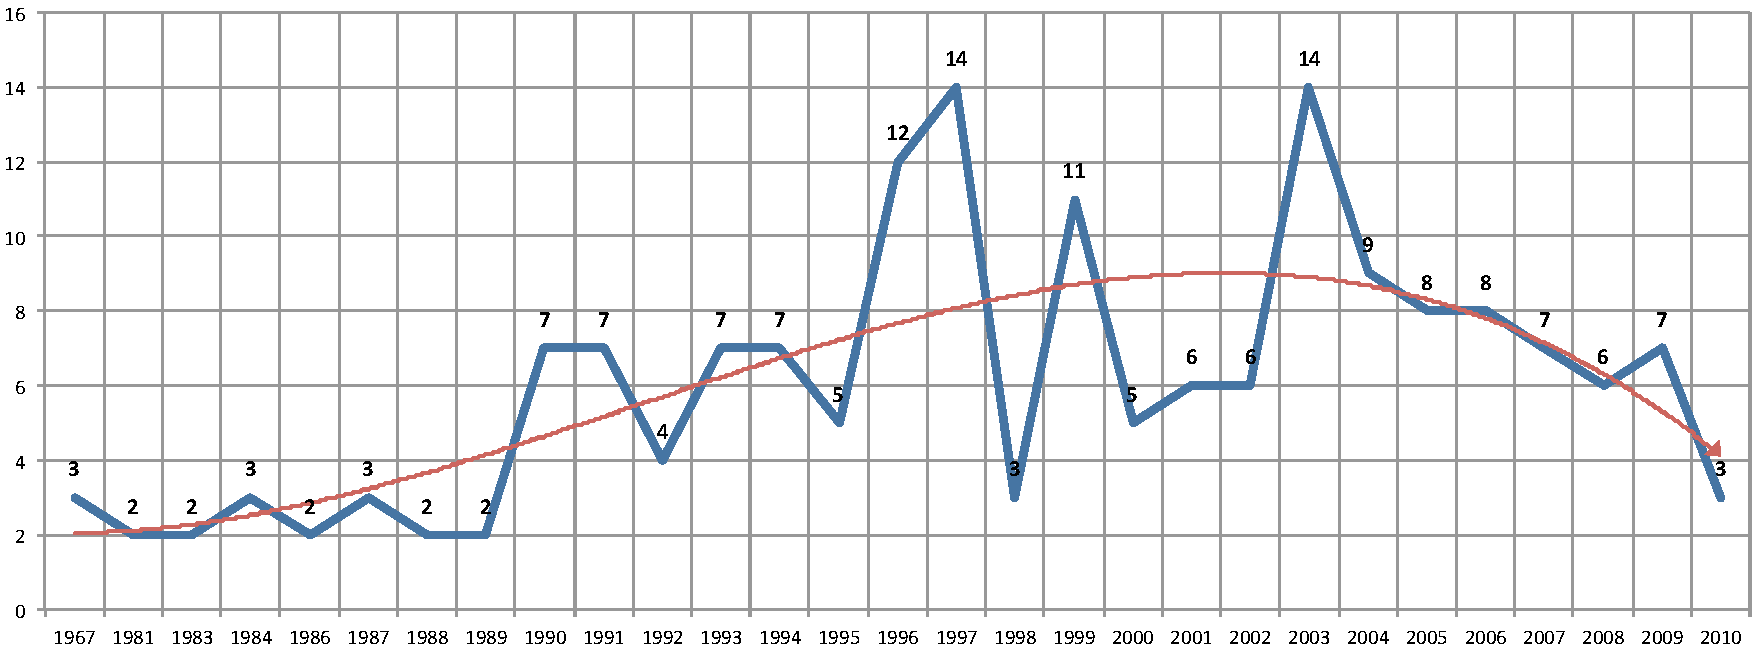
\includegraphics[scale=0.5]{abntex2-modelo-img-grafico.pdf}
	\end{center}
	\legend{Fonte: \citeonline[p. 24]{araujo2012}}
\end{figure}

% ---
\subsection{Figuras em \emph{minipages}}
% ---

\emph{Minipages} são usadas para inserir textos ou outros elementos em quadros
com tamanhos e posições controladas. Veja o exemplo da
\autoref{fig_minipage_imagem1} e da \autoref{fig_minipage_grafico2}.

\begin{figure}[htb]
 \label{teste}
 \centering
  \begin{minipage}{0.4\textwidth}
    \centering
    \caption{Imagem 1 da minipage} \label{fig_minipage_imagem1}
    
\includegraphics[scale=0.9]{abntex2-modelo-img-marca.pdf}
    \legend{Fonte: Produzido pelos autores}
  \end{minipage}
  \hfill
  \begin{minipage}{0.4\textwidth}
    \centering
    \caption{Grafico 2 da minipage} \label{fig_minipage_grafico2}
    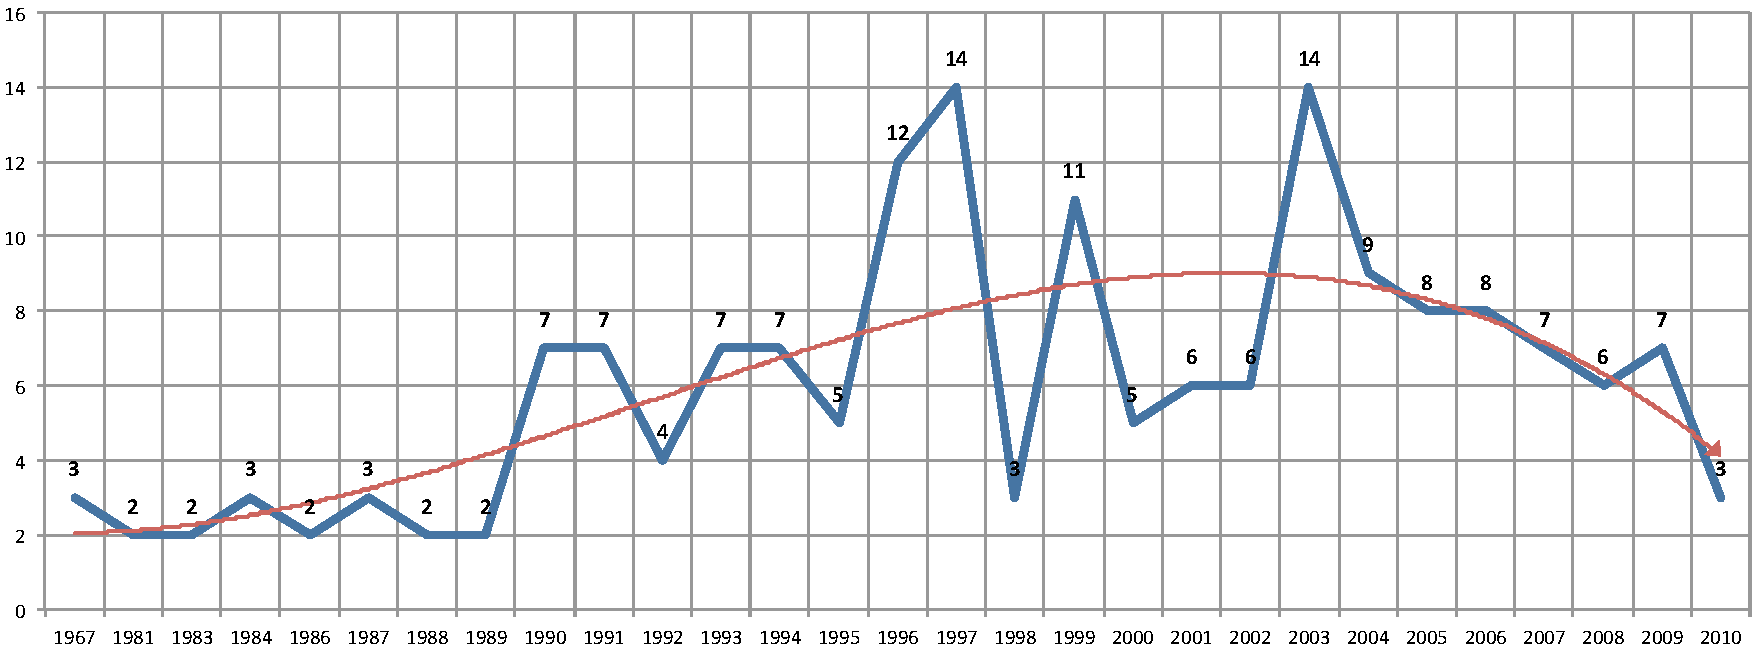
\includegraphics[scale=0.2]{abntex2-modelo-img-grafico.pdf}
    \legend{Fonte: \citeonline[p. 24]{araujo2012}}
  \end{minipage}
\end{figure}

Observe que, segundo a \citeonline[seções 4.2.1.10 e 5.8]{NBR14724:2011}, as
ilustrações devem sempre ter numeração contínua e única em todo o documento:

\begin{citacao}
Qualquer que seja o tipo de ilustração, sua identificação aparece na parte
superior, precedida da palavra designativa (desenho, esquema, fluxograma,
fotografia, gráfico, mapa, organograma, planta, quadro, retrato, figura,
imagem, entre outros), seguida de seu número de ordem de ocorrência no texto,
em algarismos arábicos, travessão e do respectivo título. Após a ilustração, na
parte inferior, indicar a fonte consultada (elemento obrigatório, mesmo que
seja produção do próprio autor), legenda, notas e outras informações
necessárias à sua compreensão (se houver). A ilustração deve ser citada no
texto e inserida o mais próximo possível do trecho a que se
refere. \cite[seções 5.8]{NBR14724:2011}
\end{citacao}

% ---
\section{Expressões matemáticas}
% ---

\index{expressões matemáticas}Use o ambiente \texttt{equation} para escrever
expressões matemáticas numeradas:

\begin{equation}
  \forall x \in X, \quad \exists \: y \leq \epsilon
\end{equation}

Escreva expressões matemáticas entre \$ e \$, como em $ \lim_{x \to \infty}
\exp(-x) = 0 $, para que fiquem na mesma linha.

Também é possível usar colchetes para indicar o início de uma expressão
matemática que não é numerada.

\[
\left|\sum_{i=1}^n a_ib_i\right|
\le
\left(\sum_{i=1}^n a_i^2\right)^{1/2}
\left(\sum_{i=1}^n b_i^2\right)^{1/2}
\]

Consulte mais informações sobre expressões matemáticas em
\url{https://github.com/abntex/abntex2/wiki/Referencias}.

% ---
\section{Enumerações: alíneas e subalíneas}
% ---

\index{alíneas}\index{subalíneas}\index{incisos}Quando for necessário enumerar
os diversos assuntos de uma seção que não possua título, esta deve ser
subdividida em alíneas \cite[4.2]{NBR6024:2012}:

\begin{alineas}

  \item os diversos assuntos que não possuam título próprio, dentro de uma mesma
  seção, devem ser subdivididos em alíneas; 
  
  \item o texto que antecede as alíneas termina em dois pontos;
  \item as alíneas devem ser indicadas alfabeticamente, em letra minúscula,
  seguida de parêntese. Utilizam-se letras dobradas, quando esgotadas as
  letras do alfabeto;

  \item as letras indicativas das alíneas devem apresentar recuo em relação à
  margem esquerda;

  \item o texto da alínea deve começar por letra minúscula e terminar em
  ponto-e-vírgula, exceto a última alínea que termina em ponto final;

  \item o texto da alínea deve terminar em dois pontos, se houver subalínea;

  \item a segunda e as seguintes linhas do texto da alínea começa sob a
  primeira letra do texto da própria alínea;
  
  \item subalíneas \cite[4.3]{NBR6024:2012} devem ser conforme as alíneas a
  seguir:

  \begin{alineas}
     \item as subalíneas devem começar por travessão seguido de espaço;

     \item as subalíneas devem apresentar recuo em relação à alínea;

     \item o texto da subalínea deve começar por letra minúscula e terminar em
     ponto-e-vírgula. A última subalínea deve terminar em ponto final, se não
     houver alínea subsequente;

     \item a segunda e as seguintes linhas do texto da subalínea começam sob a
     primeira letra do texto da própria subalínea.
  \end{alineas}
  
  \item no \abnTeX\ estão disponíveis os ambientes \texttt{incisos} e
  \texttt{subalineas}, que em suma são o mesmo que se criar outro nível de
  \texttt{alineas}, como nos exemplos à seguir:
  
  \begin{incisos}
    \item \textit{Um novo inciso em itálico};
  \end{incisos}
  
  \item Alínea em \textbf{negrito}:
  
  \begin{subalineas}
    \item \textit{Uma subalínea em itálico};
    \item \underline{\textit{Uma subalínea em itálico e sublinhado}}; 
  \end{subalineas}
  
  \item Última alínea com \emph{ênfase}.
  
\end{alineas}

% ---
\section{Espaçamento entre parágrafos e linhas}
% ---

\index{espaçamento!dos parágrafos}O tamanho do parágrafo, espaço entre a margem
e o início da frase do parágrafo, é definido por:

\begin{verbatim}
   \setlength{\parindent}{1.3cm}
\end{verbatim}

\index{espaçamento!do primeiro parágrafo}Por padrão, não há espaçamento no
primeiro parágrafo de cada início de divisão do documento
(\autoref{sec-divisoes}). Porém, você pode definir que o primeiro parágrafo
também seja indentado, como é o caso deste documento. Para isso, apenas inclua o
pacote \textsf{indentfirst} no preâmbulo do documento:

\begin{verbatim}
   \usepackage{indentfirst}      % Indenta o primeiro parágrafo de cada seção.
\end{verbatim}

\index{espaçamento!entre os parágrafos}O espaçamento entre um parágrafo e outro
pode ser controlado por meio do comando:

\begin{verbatim}
  \setlength{\parskip}{0.2cm}  % tente também \onelineskip
\end{verbatim}

\index{espaçamento!entre as linhas}O controle do espaçamento entre linhas é
definido por:

\begin{verbatim}
  \OnehalfSpacing       % espaçamento um e meio (padrão); 
  \DoubleSpacing        % espaçamento duplo
  \SingleSpacing        % espaçamento simples	
\end{verbatim}

Para isso, também estão disponíveis os ambientes:

\begin{verbatim}
  \begin{SingleSpace} ...\end{SingleSpace}
  \begin{Spacing}{hfactori} ... \end{Spacing}
  \begin{OnehalfSpace} ... \end{OnehalfSpace}
  \begin{OnehalfSpace*} ... \end{OnehalfSpace*}
  \begin{DoubleSpace} ... \end{DoubleSpace}
  \begin{DoubleSpace*} ... \end{DoubleSpace*} 
\end{verbatim}

Para mais informações, consulte \citeonline[p. 47-52 e 135]{memoir}.

% ---
\section{Inclusão de outros arquivos}\label{sec-include}
% ---

É uma boa prática dividir o seu documento em diversos arquivos, e não
apenas escrever tudo em um único. Esse recurso foi utilizado neste
documento. Para incluir diferentes arquivos em um arquivo principal,
de modo que cada arquivo incluído fique em uma página diferente, utilize o
comando:

\begin{verbatim}
   \include{documento-a-ser-incluido}      % sem a extensão .tex
\end{verbatim}

Para incluir documentos sem quebra de páginas, utilize:

\begin{verbatim}
   \input{documento-a-ser-incluido}      % sem a extensão .tex
\end{verbatim}

% ---
\section{Compilar o documento \LaTeX}
% ---

Geralmente os editores \LaTeX, como o
TeXlipse\footnote{\url{http://texlipse.sourceforge.net/}}, o
Texmaker\footnote{\url{http://www.xm1math.net/texmaker/}}, entre outros,
compilam os documentos automaticamente, de modo que você não precisa se
preocupar com isso.

No entanto, você pode compilar os documentos \LaTeX usando os seguintes
comandos, que devem ser digitados no \emph{Prompt de Comandos} do Windows ou no
\emph{Terminal} do Mac ou do Linux:

\begin{verbatim}
   pdflatex ARQUIVO_PRINCIPAL.tex
   bibtex ARQUIVO_PRINCIPAL.aux
   makeindex ARQUIVO_PRINCIPAL.idx 
   makeindex ARQUIVO_PRINCIPAL.nlo -s nomencl.ist -o ARQUIVO_PRINCIPAL.nls
   pdflatex ARQUIVO_PRINCIPAL.tex
   pdflatex ARQUIVO_PRINCIPAL.tex
\end{verbatim}

% ---
\section{Remissões internas}
% ---

Ao nomear a \autoref{tab-nivinv} e a \autoref{fig_circulo}, apresentamos um
exemplo de remissão interna, que também pode ser feita quando indicamos o
\autoref{cap_exemplos}, que tem o nome \emph{\nameref{cap_exemplos}}. O número
do capítulo indicado é \ref{cap_exemplos}, que se inicia à
\autopageref{cap_exemplos}\footnote{O número da página de uma remissão pode ser
obtida também assim:
\pageref{cap_exemplos}.}.
Veja a \autoref{sec-divisoes} para outros exemplos de remissões internas entre
seções, subseções e subsubseções.

O código usado para produzir o texto desta seção é:

\begin{verbatim}
Ao nomear a \autoref{tab-nivinv} e a \autoref{fig_circulo}, apresentamos um
exemplo de remissão interna, que também pode ser feita quando indicamos o
\autoref{cap_exemplos}, que tem o nome \emph{\nameref{cap_exemplos}}. O número
do capítulo indicado é \ref{cap_exemplos}, que se inicia à
\autopageref{cap_exemplos}\footnote{O número da página de uma remissão pode ser
obtida também assim:
\pageref{cap_exemplos}.}.
Veja a \autoref{sec-divisoes} para outros exemplos de remissões internas entre
seções, subseções e subsubseções.
\end{verbatim}

% ---
\section{Divisões do documento: seção}\label{sec-divisoes}
% ---

Esta seção testa o uso de divisões de documentos. Esta é a
\autoref{sec-divisoes}. Veja a \autoref{sec-divisoes-subsection}.

\subsection{Divisões do documento: subseção}\label{sec-divisoes-subsection}

Isto é uma subseção. Veja a \autoref{sec-divisoes-subsubsection}, que é uma
\texttt{subsubsection} do \LaTeX, mas é impressa chamada de ``subseção'' porque
no Português não temos a palavra ``subsubseção''.

\subsubsection{Divisões do documento: subsubseção}
\label{sec-divisoes-subsubsection}

Isto é uma subsubseção.

\subsubsection{Divisões do documento: subsubseção}

Isto é outra subsubseção.

\subsection{Divisões do documento: subseção}\label{sec-exemplo-subsec}

Isto é uma subseção.

\subsubsection{Divisões do documento: subsubseção}

Isto é mais uma subsubseção da \autoref{sec-exemplo-subsec}.


\subsubsubsection{Esta é uma subseção de quinto
nível}\label{sec-exemplo-subsubsubsection}

Esta é uma seção de quinto nível. Ela é produzida com o seguinte comando:

\begin{verbatim}
\subsubsubsection{Esta é uma subseção de quinto
nível}\label{sec-exemplo-subsubsubsection}
\end{verbatim}

\subsubsubsection{Esta é outra subseção de quinto nível}\label{sec-exemplo-subsubsubsection-outro}

Esta é outra seção de quinto nível.


\paragraph{Este é um parágrafo numerado}\label{sec-exemplo-paragrafo}

Este é um exemplo de parágrafo nomeado. Ele é produzida com o comando de
parágrafo:

\begin{verbatim}
\paragraph{Este é um parágrafo nomeado}\label{sec-exemplo-paragrafo}
\end{verbatim}

A numeração entre parágrafos numeradaos e subsubsubseções são contínuas.

\paragraph{Esta é outro parágrafo numerado}\label{sec-exemplo-paragrafo-outro}

Esta é outro parágrafo nomeado.

% ---
\section{Este é um exemplo de nome de seção longo. Ele deve estar
alinhado à esquerda e a segunda e demais linhas devem iniciar logo abaixo da
primeira palavra da primeira linha}
% ---

Isso atende à norma \citeonline[seções de 5.2.2 a 5.2.4]{NBR14724:2011} 
 e \citeonline[seções de 3.1 a 3.8]{NBR6024:2012}.

% ---
\section{Diferentes idiomas e hifenizações}
\label{sec-hifenizacao}
% ---

Para usar hifenizações de diferentes idiomas, inclua nas opções do documento o
nome dos idiomas que o seu texto contém. Por exemplo (para melhor
visualização, as opções foram quebras em diferentes linhas):

\begin{verbatim}
\documentclass[
	12pt,
	openright,
	twoside,
	a4paper,
	english,
	french,
	spanish,
	brazil
	]{abntex2}
\end{verbatim}

O idioma português-brasileiro (\texttt{brazil}) é incluído automaticamente pela
classe \textsf{abntex2}. Porém, mesmo assim a opção \texttt{brazil} deve ser
informada como a última opção da classe para que todos os pacotes reconheçam o
idioma. Vale ressaltar que a última opção de idioma é a utilizada por padrão no
documento. Desse modo, caso deseje escrever um texto em inglês que tenha
citações em português e em francês, você deveria usar o preâmbulo como abaixo:

\begin{verbatim}
\documentclass[
	12pt,
	openright,
	twoside,
	a4paper,
	french,
	brazil,
	english
	]{abntex2}
\end{verbatim}

A lista completa de idiomas suportados, bem como outras opções de hifenização,
estão disponíveis em \citeonline[p.~5-6]{babel}.

Exemplo de hifenização em inglês\footnote{Extraído de:
\url{http://en.wikibooks.org/wiki/LaTeX/Internationalization}}:

\begin{otherlanguage*}{english}
\textit{Text in English language. This environment switches all language-related
definitions, like the language specific names for figures, tables etc. to the other
language. The starred version of this environment typesets the main text
according to the rules of the other language, but keeps the language specific
string for ancillary things like figures, in the main language of the document.
The environment hyphenrules switches only the hyphenation patterns used; it can
also be used to disallow hyphenation by using the language name
`nohyphenation'.}
\end{otherlanguage*}

Exemplo de hifenização em francês\footnote{Extraído de:
\url{http://bigbrowser.blog.lemonde.fr/2013/02/17/tu-ne-tweeteras-point-le-vatican-interdit-aux-cardinaux-de-tweeter-pendant-le-conclave/}}:

\begin{otherlanguage*}{french}
\textit{Texte en français. Pas question que Twitter ne vienne faire une
concurrence déloyale à la traditionnelle fumée blanche qui marque l'élection
d'un nouveau pape. Pour éviter toute fuite précoce, le Vatican a donc pris un
peu d'avance, et a déjà interdit aux cardinaux qui prendront part au vote
d'utiliser le réseau social, selon Catholic News Service. Une mesure valable
surtout pour les neuf cardinaux – sur les 117 du conclave – pratiquants très
actifs de Twitter, qui auront interdiction pendant toute la période de se
connecter à leur compte.}
\end{otherlanguage*}

Pequeno texto em espanhol\footnote{Extraído de:
\url{http://internacional.elpais.com/internacional/2013/02/17/actualidad/1361102009_913423.html}}:

\foreignlanguage{spanish}{\textit{Decenas de miles de personas ovacionan al pontífice en su
penúltimo ángelus dominical, el primero desde que anunciase su renuncia. El Papa se
centra en la crítica al materialismo}}.

O idioma geral do texto por ser alterado como no exemplo seguinte:

\begin{verbatim}
  \selectlanguage{english}
\end{verbatim}

Isso altera automaticamente a hifenização e todos os nomes constantes de
referências do documento para o idioma inglês. Consulte o manual da classe
\cite{abntex2classe} para obter orientações adicionais sobre internacionalização de
documentos produzidos com \abnTeX.

A \autoref{sec-citacao} descreve o ambiente \texttt{citacao} que pode receber
como parâmetro um idioma a ser usado na citação.

% ---
\section{Consulte o manual da classe \textsf{abntex2}}
% ---

Consulte o manual da classe \textsf{abntex2} \cite{abntex2classe} para uma
referência completa das macros e ambientes disponíveis. 

Além disso, o manual possui informações adicionais sobre as normas ABNT
observadas pelo \abnTeX\ e considerações sobre eventuais requisitos específicos
não atendidos, como o caso da \citeonline[seção 5.2.2]{NBR14724:2011}, que
especifica o espaçamento entre os capítulos e o início do texto, regra
propositalmente não atendida pelo presente modelo.

% ---
\section{Referências bibliográficas}
% ---

A formatação das referências bibliográficas conforme as regras da ABNT são um
dos principais objetivos do \abnTeX. Consulte os manuais
\citeonline{abntex2cite} e \citeonline{abntex2cite-alf} para obter informações
sobre como utilizar as referências bibliográficas.

%-
\subsection{Acentuação de referências bibliográficas}
%-

Normalmente não há problemas em usar caracteres acentuados em arquivos
bibliográficos (\texttt{*.bib}). Porém, como as regras da ABNT fazem uso quase
abusivo da conversão para letras maiúsculas, é preciso observar o modo como se
escreve os nomes dos autores. Na ~\autoref{tabela-acentos} você encontra alguns
exemplos das conversões mais importantes. Preste atenção especial para `ç' e `í'
que devem estar envoltos em chaves. A regra geral é sempre usar a acentuação
neste modo quando houver conversão para letras maiúsculas.

\begin{table}[htbp]
\caption{Tabela de conversão de acentuação.}
\label{tabela-acentos}

\begin{center}
\begin{tabular}{ll}\hline\hline
acento & \textsf{bibtex}\\
à á ã & \verb+\`a+ \verb+\'a+ \verb+\~a+\\
í & \verb+{\'\i}+\\
ç & \verb+{\c c}+\\
\hline\hline
\end{tabular}
\end{center}
\end{table}


% ---
\section{Precisa de ajuda?}
% ---

Consulte a FAQ com perguntas frequentes e comuns no portal do \abnTeX:
\url{https://github.com/abntex/abntex2/wiki/FAQ}.

Inscreva-se no grupo de usuários \LaTeX:
\url{http://groups.google.com/group/latex-br}, tire suas dúvidas e ajude
outros usuários.

Participe também do grupo de desenvolvedores do \abnTeX:
\url{http://groups.google.com/group/abntex2} e faça sua contribuição à
ferramenta.

% ---
\section{Você pode ajudar?}
% ---

Sua contribuição é muito importante! Você pode ajudar na divulgação, no
desenvolvimento e de várias outras formas. Veja como contribuir com o \abnTeX\
em \url{https://github.com/abntex/abntex2/wiki/Como-Contribuir}.

% ---
\section{Quer customizar os modelos do \abnTeX\ para sua instituição ou
universidade?}
% ---

Veja como customizar o \abnTeX\ em:
\url{https://github.com/abntex/abntex2/wiki/ComoCustomizar}.


% ---

%\chapter{Conteúdos específicos do modelo de trabalho acadêmico}\label{cap_trabalho_academico}

%\section{Quadros}

%Este modelo vem com o ambiente \texttt{quadro} e impressão de Lista de quadros 
%configurados por padrão. Verifique um exemplo de utilização:

%\begin{quadro}[htb]
%\caption{\label{quadro_exemplo}Exemplo de quadro}
%\begin{tabular}{|c|c|c|c|}
%	\hline
%	\textbf{Pessoa} & \textbf{Idade} & \textbf{Peso} & \textbf{Altura} \\ \hline
%	Marcos & 26    & 68   & 178    \\ \hline
%	Ivone  & 22    & 57   & 162    \\ \hline
%	...    & ...   & ...  & ...    \\ \hline
%	Sueli  & 40    & 65   & 153    \\ \hline
%\end{tabular}
%\fonte{Autor.}
%\end{quadro}

%Este parágrafo apresenta como referenciar o quadro no texto, requisito
%obrigatório da ABNT. 
%Primeira opção, utilizando \texttt{autoref}: Ver o \autoref{quadro_exemplo}. 
%Segunda opção, utilizando  \texttt{ref}: Ver o Quadro \ref{quadro_exemplo}.

% ----------------------------------------------------------
% PARTE
% ----------------------------------------------------------
%\part{Referenciais teóricos}
% ----------------------------------------------------------

% ---
% Capitulo de revisão de literatura
% ---
\chapter{Revisão de Literatura}
% ---

% ---
\section{}
% ---


% ----------------------------------------------------------
% PARTE
% ----------------------------------------------------------
%\part{Resultados}
% ----------------------------------------------------------

% ---
% primeiro capitulo de Resultados
% ---
\chapter{Gestão do Projeto}
Esta seção detalha as principais estratégias empregadas no desenvolvimento da aplicação web de gestão para a pousada Chalés Água de Coco. Dessa forma, nela são apresentadas as metodologias, ferramentas e práticas que foram adotadas para o planejamento, execução e monitoramento do projeto, com o objetivo de garantir uma entrega organizada, eficiente e alinhada aos objetivos estabelecidos pelas partes interessadas.
% ---
% ---
\section{Organização da Equipe}
Na gestão desse projeto, a organização da equipe representou um marco fundamental e teve como foco dividir as funções e atividades necessárias para o desenvolvimento da aplicação web de gestão da pousada.
\subsection{Funções e Responsabilidades}
A designação das funções e responsabilidades foi realizada de maneira estratégica e levou em consideração as competências técnicas e experiências prévias de cada membro da equipe, visando a entrega do produto final dentro do prazo estipulado. 	A função de cada membro e suas respectivas responsabilidades estão detalhadas no quadro "\ref{quadro_funçao_responsabilidade}": Função e Responsabilidades da Equipe do Projeto.	

\begin{quadro}[htb]
	\caption{Função e Responsabilidades da Equipe do Projeto}
	\label{quadro_funçao_responsabilidade}
	\begin{tabular}{|p{2.8cm}|p{5cm}|p{7.2cm}|}
		\hline
		\textbf{Integrante} & \textbf{Função} & \textbf{Responsabilidades} \\ \hline
		Anna Julia & Analista de Cronograma & Criar e atuar na manutenção e monitoramento do cronograma do projeto, além de oferecer suporte nas práticas de gestão  \\ \hline
	
		Guilherme Akio & Engenheiro de Dados e Administrador de Banco de Dados (DBA) & Implementar, administrar  e otimizar o banco de dados da aplicação, garantindo a integridade, segurança e performance dos dados \\ \hline
	
		Guilherme \quad Bittencourt & Documentador Técnico e Engenheiro de Software & Criar e manter a documentação técnica, garantido a clareza e acessibilidade das informações do projeto. Além de definir e organizar a estrutura da aplicação.\\ \hline
	
		Kelly Radchelle & Gerente de Projeto & Coordenar a equipe e gerenciar as atividades  do projeto, a fim de facilitar as tomadas de decisões e  assegurar a comunicação entre as partes interessadas do projeto   \\ \hline
		Rafael Teixeira & Desenvolvedor Frontend e UI/UX Designer & Criar e implementar a interface da aplicação, garantindo uma boa  experiência de usuário (UX)  e design de interface (UI), além de desenvolver a lógica de apresentação.    \\ \hline
		Ricardo Carriel & Desenvolvedor Backend e Administrador de Servidores & Desenvolver a lógica de negócio da aplicação, configurar e administrar o servidor de aplicação  além de garantir a integração da aplicação  \\ \hline
	\end{tabular}
	\fonte{Elaborado pelos autores.}
\end{quadro}
%---
%---
\section{Metodologias de gestão e desenvolvimento}
Para assegurar que o produto final seja entregue em pleno alinhamento com as expectativas da cliente, a equipe envolvida no projeto optou pela adoção da metodologia ágil Scrum como ferramenta de gestão e desenvolvimento do projeto. Essa decisão fundamentou-se na familiaridade da equipe com a estrutura, na capacidade do Scrum de otimizar a organização, divisão e planejamento de atividades do projeto, e em sua relevância como framework de gerenciamento– dado seu uso extensivo no contexto de desenvolvimento de softwares complexos.
Segundo Schwaber e Sutherland (2020), o Scrum é um framework estruturado desenvolvido na década de 1990. Ele foi criado com o intuito de auxiliar equipes na criação e gerenciamento de produtos complexos. Para isso o Scrum tem como pilares fundamentais a transparência, a inspeção e a adaptação. A transparência garante que todos os aspectos significativos do processo estejam visíveis e claros para as partes interessadas a todo momento. A inspeção envolve o acompanhamento regular dos artefatos e progresso, a fim da detecção precoce de problemas. Por fim, a adaptação refere-se à capacidade de fazer ajustes no processo  em resposta aos problemas anteriormente detectados na inspeção, com o objetivo de otimizar os resultados.
Sabendo que para operacionalizar esses pilares e assegurar um ciclo de desenvolvimento iterativo e incremental, a metodologia Scrum sugere a definição de papeis específicos dentro do time, estabelece a realização de uma sequência de eventos formais e o uso de artefatos específicos, os integrantes da equipe desenvolveram as tarefas e eventos sugeridos pelo Scrum para a gestão e desenvolvimento do projeto.

\subsection{Time Scrum}
Como estabelecido no Guia do Scrum (SCHWABER; SUTHERLAND, 2020), os membros da equipe do projeto assumem papeis específicos que compõem um time Scrum: Dono do Produto (Product Owner), Scrum Master e Time de Desenvolvimento. 
O Dono do Produto (Product Owner) é o representante das partes interessadas (Stakeholders) e tem como responsabilidade principal gerenciar o backlog do Produto, a fim de maximizar o valor do produto e otimizar o trabalho do Time de Desenvolvimento. 
O Scrum Master é o responsável por promover e facilitar a aplicação da teoria e das práticas do framework, atuando como um líder-servidor ao auxiliar a equipe na retirada de impedimentos que venham afetar seu progresso . 
O Time de Desenvolvimento é responsável por entregar um incremento (versão potencialmente usável do produto) ao final de cada sprint, atuando de maneira auto-organizada e multifuncional . 
Ciente disso, realizou-se a distribuição dos papeis de um time scrum entre os integrantes da equipe e registrou-se na “\autoref{tab:time_scrum}”.

\begin{table}[htb]
	\centering
	\caption{Função dos Integrantes da Equipe}
	\label{tab:time_scrum}
	\begin{tabular}{|c|c|c|c|}
		\hline
		\textbf{Integrante} & \multicolumn{3}{c|}{\textbf{Função}} \\ \cline{2-4}
		& \textit{Product Owner} & \textit{Scrum Master} & \textit{Time de Desenvolvimento} \\ \hline
		Anna Julia & X & & \\ \hline
		Guilherme Akio & & & X \\ \hline
		Guilherme Bittencourt & & & X \\ \hline
		Kelly Radchelle & X & & \\ \hline
		Rafael Teixeira & & & X \\ \hline
		Ricardo Carriel & & & X \\ \hline
	\end{tabular}
	\fonte{Elaborado pelos autores.}
\end{table}
%---

%---
\section{Artefatos}
No scrum,  os artefatos são elementos fundamentais que ajudam a equipe a consolidar a transparência no processo de desenvolvimento. Cientes das suas importâncias, o time scrum realizou o planejamento inicial dos artefatos: Product Backlog e Sprints Backlog.

\subsection{Product Backlog}
O Product Backlog consiste em uma lista ordenada de todos os itens de trabalho, sendo elas as funcionalidades, os requisitos e os aprimoramentos necessários para a produção do produto,  e que oferecem o máximo valor e utilidade para o cliente. Diante disso, foi elaborado pelo product owner o backlog de produto inicial do projeto da aplicação web de gestão da pousada Chalés Água de Coco (\autoref{}) com base nas histórias de usuário levantadas pela equipe, visto que, elas expressam as necessidades e expectativas sob a perspectiva da usuária e principal stakeholder.

\begin{quadro}[htb]
	\caption{Product backlog}
	\label{quadro_product_backlog}
	\begin{tabular}{|c|c|c|c|}
		\hline
		\textbf{Ordem} & \textbf{Item} & \textbf{Domínio} & \textbf{Prioridade} \\ \hline
		1 & Configurar ambiente de hospedagem & Infraestrutura e Configuração   & Essencial    \\ \hline
		2 & Configurar repositório Git e fluxo de versionamento & Infraestrutura e Configuração & Essencial  \\ \hline
		3 & ...   & ...  & ...    \\ \hline
		4 & 40    & 65   & 153    \\ \hline
		5 & 40    & 65   & 153    \\ \hline
		6 & 40    & 65   & 153    \\ \hline
		7 & 40    & 65   & 153    \\ \hline
		8 & 40    & 65   & 153    \\ \hline
		9 & 40    & 65   & 153    \\ \hline
		10 & 40    & 65   & 153    \\ \hline
	\end{tabular}
	\fonte{Autor.}
\end{quadro}
% ---


% ---
% segundo capitulo de Resultados
% ---
\chapter{Desenvolvimento do Projeto}
\section{Escopo do Projeto}
\subsection{Requisitos Funcionais}
\begin{quadro}[H]
	\caption{Requisitos Funcionais - Parte 1}
	\label{quadro_rf1}
	\begin{tabular}{|c|p{5cm}|c|p{4cm}|}
		\hline
		\textbf{Código} & \textbf{Descrição} & \textbf{Prioridade} & \textbf{Regra de Negócio} \\ \hline
		RF01 & O sistema deve permitir o cadastro de reservas, associando um quarto a um período (data de check-in e check-out) & Alta & Não Aplicável \\ \hline
		RF02 & O sistema deve permitir o cadastro de reservas, associando um quarto a um período (data de check-in e check-out) & Alta & RN03, RN01 \\ \hline
		RF03 & Uma reserva deve estar associada a um quarto disponível para que ela seja cadastrada. & Alta & RN11 \\ \hline
		RF04 & O sistema deve exigir os dados pessoais do hóspede para que a reserva seja cadastrada: nome completo, endereço completo, CPF, telefone e e-mail. & Alta & RN05 \\ \hline
		RF05 & A proprietária deve conseguir reservar quartos para um cliente em nome de outra pessoa responsável, registrando os dados do hóspede e, opcionalmente, do responsável. & Média & RN06 \\ \hline
		RF06 & O sistema deve exigir o pagamento de 50 por cento do valor da estadia para confirmar o cadastro da reserva (a ser pago no momento da reserva ou em um prazo definido). & Média & RN01 \\ \hline
		RF07 & O sistema deve permitir o registro da comprovação do pagamento & Média & RN01 \\ \hline
	\end{tabular}
	\fonte{Elaborado pelos autores.}
\end{quadro}

\begin{quadro}[H]
	\caption{Requisitos Funcionais - Parte 2}
	\label{quadro_rf2}
	\begin{tabular}{|c|p{5cm}|c|p{4cm}|}
		\hline
		\textbf{Código} & \textbf{Descrição} & \textbf{Prioridade} & \textbf{Regra de Negócio} \\ \hline
		RF08 & A proprietária deve conseguir cancelar ou remarcar uma reserva, com possível registro do motivo & Média & RN02 \\ \hline
		RF09 & A proprietária deve poder visualizar todas as reservas, com detalhes do hóspede, quarto reservado e período & Alta & RN15 \\ \hline
		RF10 & A proprietária deve conseguir cadastrar mais de uma reserva no nome de um mesmo cliente & Média & RN04 \\ \hline
		RF11 & A proprietária deve conseguir reservar um mesmo quarto para diferentes clientes em datas seguidas respeitando os horários de check-in e check-out configurados para quarto & Alta & RN11 \\ \hline
		RF12 & A proprietária deve conseguir acessar o histórico de reservas de um cliente & Média & RN15 \\ \hline
		RF13 & O sistema deve mudar o status do quarto para ocupado após a realização do check-in & Alta & Não Aplicável \\ \hline
		RF14 & O sistema mandar deve uma notificação para o hospede após a confirmação da reserva & Baixa & Não Aplicável \\ \hline
	\end{tabular}
	\fonte{Elaborado pelos autores.}
\end{quadro}
\begin{quadro}[H]
	\caption{Requisitos Funcionais - Parte 3}
	\label{quadro_rf3}
	\begin{tabular}{|c|p{5cm}|c|p{4cm}|}
		\hline
		\textbf{Código} & \textbf{Descrição} & \textbf{Prioridade} & \textbf{Regra de Negócio} \\ \hline
		RF15 & O sistema deve permitir o cadastro de novos quartos, incluindo informações como número/nome do quarto, capacidade (número de hóspedes) tipo (ex: chale, simples solteiro, simples casal, etc.), e preço por noite. & Alta & Não Aplicável \\ \hline
		RF16 & A proprietária deve conseguir editar as informações dos quartos já cadastrados & Alta & Não Aplicável \\ \hline
		RF17 & A proprietária deve poder visualizar todos os quartos cadastrados. & Alta & Não Aplicável \\ \hline
		RF18 & O sistema deve permitir a visualização dos quartos disponíveis no período de tempo selecionado para a reserva & Média & RN03, RN11 \\ \hline
		RF19 & A proprietária deve conseguir mudar c status de um quarto (ex: disponível, indisponível, em manutenção). & Alta & RN10 \\ \hline
	\end{tabular}
	\fonte{Elaborado pelos autores.}
\end{quadro}
\begin{quadro}[H]
	\caption{Requisitos Funcionais - Parte 4}
	\label{quadro_rf4}
	\begin{tabular}{|c|p{5cm}|c|p{4cm}|}
		\hline
		\textbf{Código} & \textbf{Descrição} & \textbf{Prioridade} & \textbf{Regra de Negócio} \\ \hline
		RF20 & A proprietária deve poder registrar as despesas da pousada, categorizando-as (ex manutenção, limpeza, contas de consumo), especificando a data, o valor, a categoria e uma descrição da despesa & Média & Não Aplicável \\ \hline
		RF21 & A proprietária deve conseguir cadastrar gastos fixos e gastos variáveis. & Média & Não Aplicável \\ \hline
		RF22 & A proprietária deve poder registrar receitas, associando-as a uma reserva ou a outras fontes de receita, especificando a data, o valor e uma descrição da receita. & Média & RN13 \\ \hline
		RF23 & O sistema deve permitir que a proprietária visualize todas as transações financeiras (receitas e despesas) em um determinado período. & Média & Não Aplicável \\ \hline
		RF24 & O sistema deve permitir a filtragem das transações por tipo (receita/despesa), data e categoria & Média & Não Aplicável \\ \hline
		RF25 & O sistema deve ser capaz de gerar um balanço financeiro simples para um período selecionado, mostrando o total de receitas, o total de despesas e o saldo & Média & Não Aplicável \\ \hline
	\end{tabular}
	\fonte{Elaborado pelos autores.}

\end{quadro}
\subsection{Requisitos Não Funcionais}
\begin{quadro}[H]
	\caption{\label{quadro_rnf1}Requisitos Não Funcionais - Parte 1}
	\begin{tabular}{|c|p{4cm}|p{8cm}|}
		\hline
		\textbf{Código} & \textbf{Módulo} & \textbf{Descrição} \\ \hline
		RNF01 & Usabilidade & A interface do sistema deve ser intuitiva, responsiva (compatível e adaptada tanto para dispositivos desktop quanto mobile) e de fácil utilização, de modo que as tarefas essenciais da gestão da pousada sejam realizadas de forma eficiente e com mínimo esforço de aprendizado pela proprietária. Para isso, deve-se adotar os princípios de interface amigável como a priorização da simplicidade e da clareza, padrões de interface consistentes e acessíveis. \\ \hline
		RNF02 & Usabilidade & O sistema deve fornecer mensagens de feedback claras, objetivas e contextualizadas para todas as ações realizadas pela usuária, como confirmação de reserva (exemplo: reserva efetuada com sucesso) ou notificações de erros (exemplo: falha ao cadastrar um quarto), garantindo uma interação segura e satisfatória. \\ \hline
		RNF03 & Performance & O sistema deve apresentar um tempo de resposta baixo, com carregamento das páginas e execução de ações da proprietária entre 2 e 3 segundos, para garantir uma navegação fluida. \\ \hline
		RNF04 & Performance & O sistema deve ser capaz de lidar com a carga de trabalho estimada desde o registro e a consulta simultânea de dados à gestão de múltiplas reservas, sem degradação significativa no desempenho, este que deverá se manter estável mesmo em períodos de maior demanda, considerando o perfil sazonal do negócio. \\ \hline
		RNF05 & Segurança & O sistema deve garantir a segurança das informações da pousada e dos hóspedes através da implementação de mecanismos robustos de autenticação e autorização, de forma a assegurar que apenas a usuária autorizada consiga acessar ou alterar dados na aplicação. \\ \hline
	
	\end{tabular}
	\fonte{Elaborado pelos autores.}
\end{quadro}
\begin{quadro}[H]
	\caption{\label{quadro_rnf2}Requisitos Não Funcionais - Parte 2}
	\begin{tabular}{|c|p{4cm}|p{8cm}|}
		\hline
		\textbf{Código} & \textbf{Módulo} & \textbf{Descrição} \\ \hline
		RNF06 & Segurança & Os dados sensíveis devem ser protegidos conforme as melhores práticas propostas pela LGPD (Lei Geral de Proteção de Dados Pessoais), incluindo: utilização de criptografia para proteger dados em trânsito (HTTPS) e em repouso, implementação de políticas de autenticação robusta e minimização da coleta de dados. \\ \hline
		RNF07 & Confiabilidade & O sistema deve estar disponível e funcionando corretamente por pelo menos 99 por cento do tempo, a fim de garantir que a proprietária tenha acesso ao sistema sempre que necessário, inclusive nos períodos com maior movimento de hóspedes na pousada. \\ \hline
		RNF08 & Confiabilidade & O sistema deve implementar mecanismos de tratamento de erros para que falhas e perdas de dados sejam prevenidas. \\ \hline
		RNF09 & Confiabilidade & O deploy da aplicação deve ser realizado em uma infraestrutura de nuvem (Amazon EC2), a fim de proporcionar maior estabilidade, flexibilidade à aplicação e permitir que possíveis atualizações e manutenções tenham impacto mínimo para a usuária. \\ \hline
		RNF10 & Escalabilidade & Embora o sistema, inicialmente, seja voltado para uma única usuária, a arquitetura deve ser projetada de forma a permitir futuras expansões no número de usuários e funcionalidades sem grandes refatorações. \\ \hline
		RNF11 & Documentação & O sistema deve possuir uma documentação completa, objetiva e atualizada, incluindo código-fonte, a arquitetura da aplicação, os fluxos de uso e as especificações de APIs possivelmente integradas. \\ \hline
		RNF12 & Documentação & A documentação deve estar versionada e organizada em no repositório Git — o GitHub —, este que deve ser utilizado no controle de versão da aplicação e colaboração entre os membros da equipe. \\ \hline
		RNF13 & Documentação & O desenvolvimento deve seguir as boas práticas de codificação e padrões recomendados para aplicações Django, a fim de assegurar a manutenibilidade, extensibilidade e integridade do sistema ao longo do seu ciclo de vida. \\ \hline
	\end{tabular}
	\fonte{Elaborado pelos autores.}
\end{quadro}




\subsection{Regras de Negócio}
\begin{quadro}[H]
	\caption{\label{quadro_rn}Regras de Negócio}
	\begin{tabular}{|c|p{8cm}|}
	\hline
	\textbf{Regra} & \textbf{Descrição}  \\ \hline	
	RN01 & A confirmação de uma reserva deve ocorrer mediante o pagamento de 50 por cento do valor total.   \\ \hline
	RN02 & Cancelamentos e remarcações são permitidos, sujeitos a regras e taxas específicas.   \\ \hline
	RN03 & As reservas devem ser registradas com, no mínimo, 2 dias de antecedência da data de entrada.  \\ \hline
	RN04 & Um mesmo hóspede pode ter mais de uma reserva ativa.   \\ \hline
	RN05 & Para efetuar uma reserva, os seguintes dados do hóspede são obrigatórios: nome completo, endereço completo, CPF, telefone e e-mail   \\ \hline
	RN06 & Um responsável pode realizar reservas em nome de outros hóspedes.   \\ \hline
	RN07 & Um responsável pode realizar reservas em nome de outros hóspedes.   \\ \hline
	RN08 & Os horários padrão são: check-in das 16h às 22h; check-out das 8h às 14h.   \\ \hline
	RN09 & A emissão de recibos ou comprovantes após check-in/out não é obrigatória.   \\ \hline
	RN10 & Um quarto pode ficar indisponível para manutenção.   \\ \hline
	RN11 & É permitido reservar um mesmo quarto para hóspedes diferentes em datas seguidas.   \\ \hline
	RN12 & Atualmente, não há oferta de serviços adicionais vinculados à reserva.   \\ \hline
	RN13 & São aceitas as formas de pagamento: Pix, dinheiro e cartão (com taxa da operadora).   \\ \hline
	RN14 & Deve ser enviada a confirmação da reserva para o cliente com todos os dados necessários.   \\ \hline
	RN15 & Apenas a proprietária deve acessar as informações dos hóspedes e reservas.   \\ \hline
\end{tabular}
\fonte{Elaborado pelos autores.}
\end{quadro}



\section{História de Usuário}
\subsection{Descrição}

\section{Arquitetura}
\subsection{Desenho da Arquitetura}
A arquitetura do sistema foi criada para atender às necessidades de um ambiente web moderno, seguro e escalável, com foco na praticidade do uso para a gestora da pousada.

A aplicação adota o padrão MTV (Model-Template-View), próprio do framework Django, no qual a separação entre dados, lógica de apresentação e lógica de negócio é claramente definida. Esse padrão proporciona uma estrutura organizada, facilitando tanto a manutenção quanto a adição de novas funcionalidades ao longo do tempo.

No front-end, a aplicação utiliza templates HTML integrados às views do Django, o que permite a criação de páginas dinâmicas. Os dados vindos do back-end são inseridos diretamente nos templates, tornando a navegação mais fácil, sem a necessidade de frameworks.

O back-end é totalmente desenvolvido com o framework Django, em Python, onde são tratadas as requisições, regras de negócio e persistência de dados. O Django oferece um conjunto de ferramentas prontas que aumentam a produtividade no desenvolvimento e garantem a segurança da aplicação.

Para o banco de dados, foi escolhido o PostgreSQL, compatível com o Django, sendo ideal para armazenar as reservas, dados de hóspedes, acomodações e demais informações do sistema.

A aplicação está hospedada na Amazon Web Services (AWS), a escolha dela se deu por sua alta disponibilidade, segurança avançada, escalabilidade sob demanda e facilidade de integração com outras ferramentas. Dentre os serviços da AWS utilizados, destacam-se:
Amazon EC2, para hospedagem da aplicação Django;
Amazon RDS (PostgreSQL), para o banco de dados gerenciado;
Amazon S3, para armazenamento de arquivos estáticos e mídias;
AWS Backup e Monitoramento, para garantir segurança e integridade dos dados.

A arquitetura permite que o sistema cresça ao longo do tempo, incorporando novos módulos e funcionalidades como integração com gateways de pagamento, envio automático de e-mails, e etc, mantendo a manutenibilidade, segurança e eficiência como foco do projeto.

\subsection{Diagrama da Arquitetura}
\subsubsection{Diagrama de Implantação}
A Figura~\ref{fig:diagramaimplantação} mostra o funcionamento da arquitetura do sistema.

\begin{figure}[H]
	\centering
	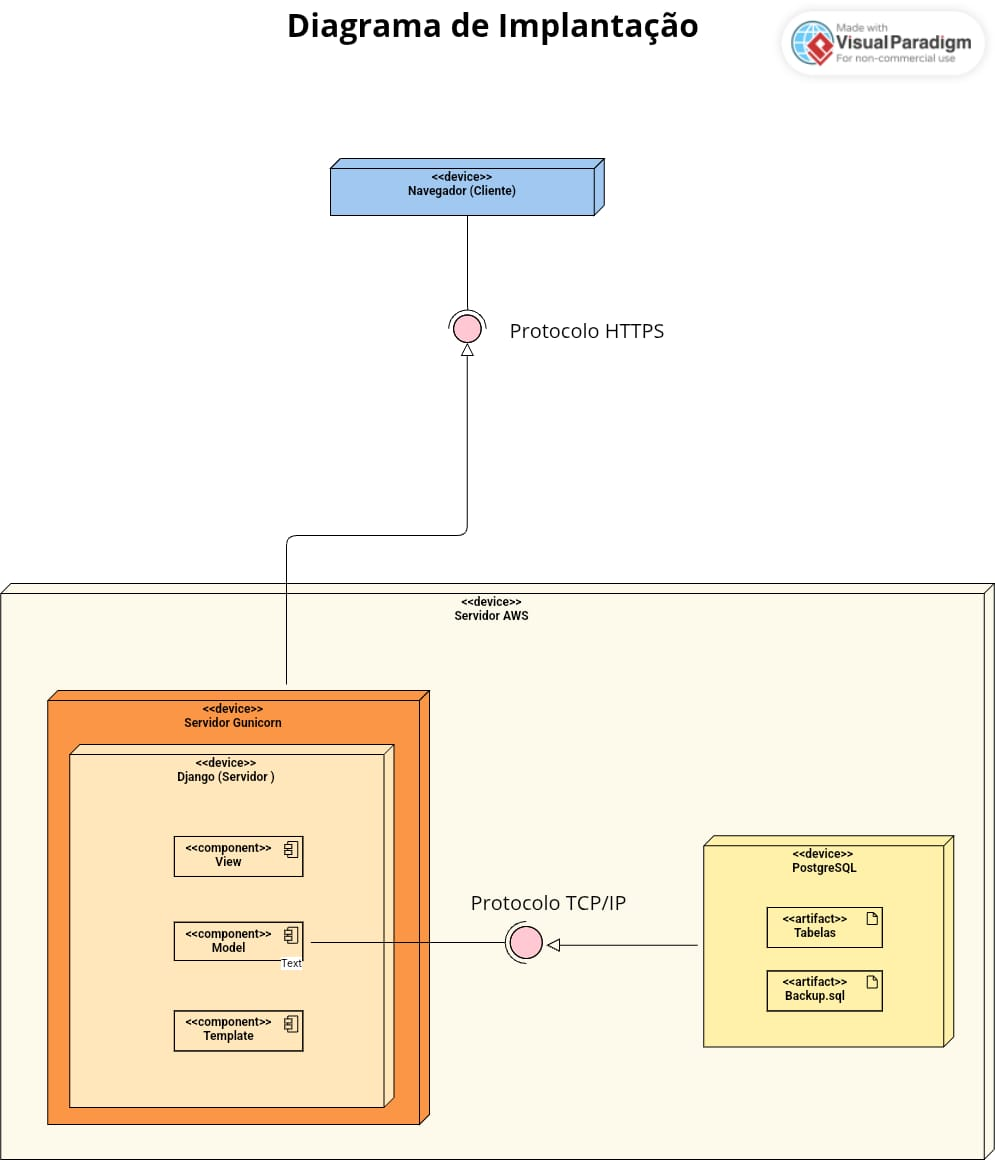
\includegraphics[width=\textwidth]{Diagrama de Implantação- Digitalização da Pousada.JPEG}
	\caption{Diagrama de Implantação desenvolvido no Online Visual-Paradigm}
	\label{fig:diagramaimplantação}
\end{figure}
\subsubsection{Diagrama de Componentes}
A Figura~\ref{fig:diagramacomponentes} mostra o funcionamento da arquitetura do sistema.

\begin{figure}[h!]
	\centering
	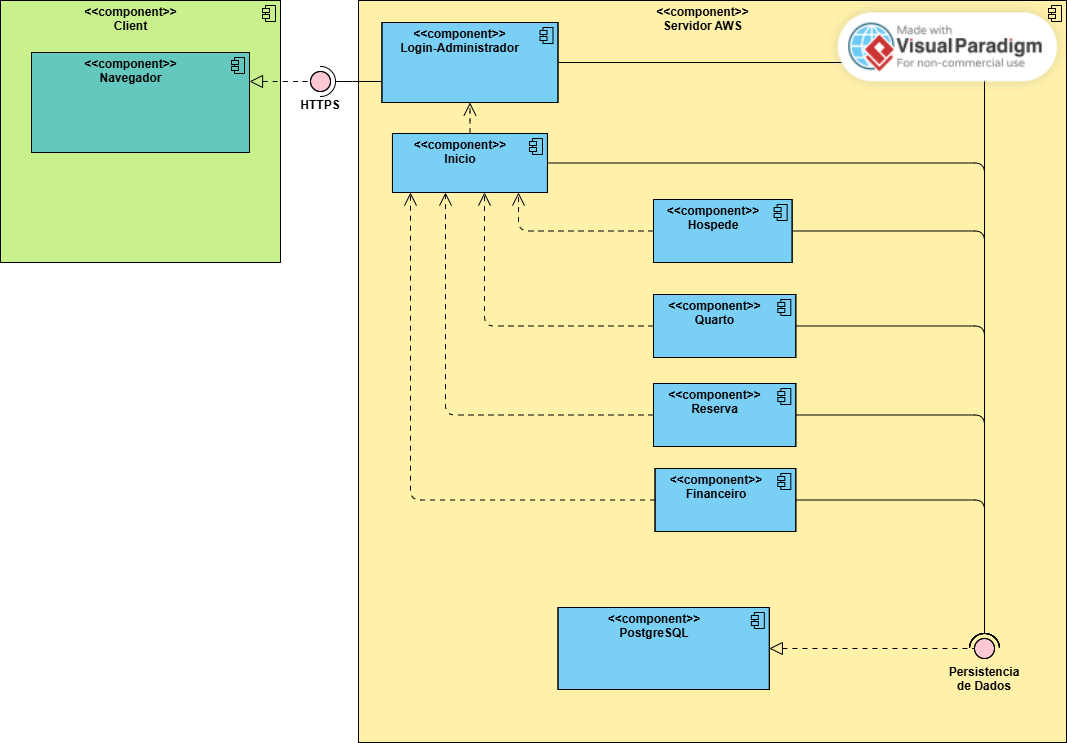
\includegraphics[width=\textwidth]{0406-Componentes.png}
	\caption{Diagrama de Componentes desenvolvido no Online Visual-Paradigm}
	\label{fig:diagramacomponentes}
\end{figure}


\section{Tecnologias}
\subsection{Front-End}
O Django é um framework web de alto nível baseado em Python que oferece uma série de recursos que o tornam ideal para o desenvolvimento de sistemas como o nosso gerenciador de reservas de quartos. Uma de suas principais vantagens é a rapidez no desenvolvimento, já que ele vem com diversas funcionalidades já prontas.

O desenvolvimento do Frond-end da aplicação Chalés Água de Coco se dá pela combinação de templates HTML associados a Views (Django) para gerar páginas dinâmicas. Os templates exibem essas informações de forma estruturada na interface do usuário, permitindo que elementos HTML sejam preenchidos com dados fornecidos pelo servidor, assim utilizando o padrão MTV (Model-Template-View).

O que facilita a manutenção e a escalabilidade do sistema. Isso é essencial em um sistema de reservas, que pode crescer em funcionalidades como calendário de disponibilidade, gestão de hóspedes, geração de relatórios, envio de notificações, entre outros.
\subsection{Back-End}
O desenvolvimento do back-end desta aplicação Django é baseada no padrão MTV(Model-Template-View), assim funcionando com manipulação de dados e lógica de negócio através das Views, que são responsáveis por processar requisições, acessar o banco de dados e enviar informações para os templates.

Outro ponto importante que influenciou na nossa escolha é a segurança, pois o Django já vem com proteções contra ataques comuns, como injeção de SQL, o que é essencial em aplicações que lidam com dados pessoais e financeiros dos clientes.
\subsection{Banco de Dados}
O Banco de Dados escolhido para esta aplicação foi o PostgreSQL, sendo um banco escalável e flexível, este SGBD pode suportar grandes volumes de dados e de usuários além de ser compatível com uma grande gama de linguagens de programação.
O PostgreSQL também é uma ótima opção por ser acessível, já que sua licença é livre, assim sem custos de licenciamento e a liberdade para modificar ou implementar o código-fonte da maneira que for necessária.
\subsection{Infraestrutura}
Agora falando um pouco sobre a Amazon Web Services. Ela é uma das plataformas de computação em nuvem mais completas e confiáveis do mercado. Utilizar a AWS para hospedar nosso sistema de gerenciamento de reservas traz várias vantagens:

Alta disponibilidade e escalabilidade: a AWS permite escalar a infraestrutura de acordo com a demanda, garantindo que o sistema continue funcionando bem mesmo em períodos de alta procura.

Confiabilidade e desempenho: a infraestrutura da AWS é robusta, distribuída globalmente e projetada para evitar falhas. Isso assegura que o sistema fique no ar com alta performance e baixa latência.

Segurança: a AWS oferece diversas camadas de segurança, incluindo criptografia de dados, controle de acesso, backups automatizados e monitoramento contínuo, protegendo tanto os dados dos hóspedes quanto as informações administrativas da pousada.

Serviços integrados: além do serviço de hospedagem, a AWS oferece bancos de dados gerenciados, armazenamento, envio de e-mails, monitoramento, entre outros — todos integráveis com o sistema Django de forma eficiente.

Por conta desses motivos, nós concluímos que a combinação de Django com a AWS é uma escolha estratégica e poderosa para o desenvolvimento do nosso sistema de reservas de quartos em uma pousada. Enquanto o Django acelera o desenvolvimento e garante um sistema seguro e bem estruturado, a AWS fornece a base tecnológica para garantir desempenho, estabilidade e escalabilidade. Juntos, eles possibilitam a entrega de uma solução profissional e confiável, algo que nós buscamos para o desenvolvimento do nosso sistema.

\section{Ferramentas de Apoio}
\subsection{GitHub}
O GitHub foi utilizado para controle de versão e colaboração durante o desenvolvimento do sistema. A plataforma permite armazenar e gerenciar o código-fonte, realizar revisões e integrar funcionalidades de forma eficiente. O GitHub facilitou a organização do fluxo de trabalho, o rastreamento de mudanças e a colaboração entre os membros da equipe, promovendo maior controle e transparência no ciclo de desenvolvimento.
\subsection{BRModelo}
O BRModelo foi utilizado para a modelagem lógica e relacional do banco de dados. A ferramenta oferece uma interface intuitiva para construção de diagramas entidade-relacionamento (DER), o que auxiliou na estruturação clara das tabelas, relacionamentos e chaves do sistema. O uso do BRModelo contribuiu diretamente para a coerência e integridade do esquema de dados implementado no PostgreSQL.
\subsection{Visual Paradigm Online}
O Visual Paradigm Online foi utilizado na criação dos diagramas de Implantação e Componentes. Esta ferramenta auxiliou na documentação da arquitetura do sistema, contribuindo para uma melhor compreensão dos fluxos e interações entre os componentes. A versão online possibilitou colaboração remota e armazenamento em nuvem, o que otimizou a produtividade da equipe.
\subsection{Latex}
O LaTeX foi utilizado na produção e formatação do trabalho acadêmico. Por meio de seu sistema de marcação, foi possível obter um alto nível de controle sobre a estrutura e apresentação do documento, garantindo consistência, qualidade e organização.

\subsection{Google Meet}
O Google Meet foi utilizado como plataforma de comunicação e realização de encontros virtuais da equipe ao longo do desenvolvimento do projeto. As reuniões periódicas possibilitaram a discussão de tarefas, alinhamento de prazos e entregas mais organizadas.

\section{Manutenibilidade}
A manutenibilidade do sistema de reservas para pousadas desenvolvido neste projeto é assegurada por meio de práticas estruturadas de engenharia de software, que facilitam a correção de erros, inclusão de novas funcionalidades e adaptação a futuras necessidades.

O sistema foi concebido com uma arquitetura modular, respeitando os princípios de separação de responsabilidades. Isso permite que diferentes partes do sistema, como interface, regras de negócio e persistência de dados, sejam modificadas de forma independente, minimizando impactos colaterais e reduzindo o tempo de manutenção.

Além disso, foram adotados padrões de codificação consistentes e bem documentados, com o intuito de facilitar a leitura e compreensão do código por outros desenvolvedores. Esses padrões promovem a reutilização e a extensibilidade do sistema.

A utilização do sistema de controle de versão Git, em conjunto com a plataforma GitHub, possibilita o rastreamento detalhado de alterações, revisão de código e colaboração eficaz entre os membros da equipe. Isso garante maior controle sobre o histórico de desenvolvimento e facilita a identificação e resolução de falhas.

A aplicação também contará com testes automatizados, cobrindo os principais fluxos da aplicação, como testes unitários para funções críticas e testes de integração entre os módulos.

Complementando essas práticas, será elaborada uma documentação técnica e funcional completa, abrangendo instruções de uso, instalação, configuração e manutenção.

Por fim, o projeto segue um ciclo de desenvolvimento bem definido, com etapas de planejamento, codificação, testes, implantação e manutenção. Essa abordagem estruturada proporciona maior previsibilidade, qualidade e agilidade na evolução contínua da aplicação, assegurando sua longevidade e adaptabilidade.

\section{Segurança, Privacidade e Legislação}
A segurança da informação é um aspecto central no desenvolvimento do sistema da Pousada Chalés Água de Coco. Para garantir a proteção dos dados dos hospedes e da própria aplicação, foi adotado o framework Django, que já incorpora diversas camadas de segurança por padrão. Além disso, foram implementadas boas práticas relacionadas à privacidade e à conformidade com a legislação brasileira de proteção de dados.

O Django fornece mecanismos robustos contra ataques comuns na web, como injeção de SQL, execução remota de código, ataques Cross-Site Scripting (XSS) e falsificação de requisições entre sites (CSRF). Essas proteções são ativadas por padrão e complementadas com práticas adicionais durante o desenvolvimento.

Entre os recursos utilizados, destacam-se:

Sistema de autenticação integrado: O Django oferece um módulo completo para autenticação e autorização de usuários, permitindo o controle de acesso baseado em permissões. O sistema foi configurado para exigir credenciais válidas e proteger páginas sensíveis com autenticação obrigatória.

Proteção contra CSRF (Cross-Site Request Forgery): Todas as requisições POST são protegidas por tokens CSRF, garantindo que ações críticas só possam ser executadas por usuários autenticados a partir da própria aplicação.

Escapamento automático de HTML (XSS): O mecanismo de templates do Django realiza automaticamente o escapamento de dados inseridos pelos usuários, o que impede a execução de scripts maliciosos.

Hash de senhas com algoritmos seguros: As senhas dos usuários são armazenadas de forma segura com algoritmos de hash modernos (como PBKDF2), tornando inviável a recuperação das senhas mesmo em caso de vazamento da base de dados.

Validação de entradas e uso de ORM: Ao utilizar o ORM (Object-Relational Mapper) do Django, o sistema evita o uso direto de comandos SQL, o que mitiga o risco de injeção de código malicioso no banco de dados.

Gerenciamento de sessões seguro: O Django gerencia sessões de forma criptografada e armazena os identificadores de sessão com proteção contra falsificação. O sistema pode ser configurado para expirar sessões inativas e exigir reautenticação para operações sensíveis.

Além dessas funcionalidades nativas, o sistema conta com certificado SSL/TLS para garantir a criptografia do tráfego entre cliente e servidor, além de backups automáticos armazenados na nuvem (AWS), oferecendo resiliência em caso de falhas técnicas.

\subsection{Conformidade com a LGPD}
Para atender à Lei Geral de Proteção de Dados (LGPD - Lei nº 13.709/2018), o sistema foi desenvolvido com foco na coleta mínima de dados, transparência e controle por parte do usuário. As finalidades de uso das informações são claramente definidas, e o usuário pode, a qualquer momento, solicitar a remoção de seus dados ou a revisão do consentimento.

Com isso, o sistema não apenas assegura uma navegação segura e confiável, mas também respeita os direitos fundamentais de privacidade e liberdade informacional previstos na legislação brasileira.

\subsection{Protocolos de Segurança na Comunicação}
A segurança na troca de informações no sistema “Chalés Água de Coco” foi uma prioridade desde as fases iniciais de desenvolvimento. Para garantir a integridade, a confidencialidade e a autenticidade dos dados transmitidos, adotaram-se protocolos amplamente reconhecidos e confiáveis no ambiente web moderno.

\subsubsection{Certificação Digital com SSL/TLS}
A aplicação foi implementada com suporte ao protocolo TLS (Transport Layer Security), sucessor do SSL, por meio de certificado digital instalado no servidor web em nuvem (AWS). Este certificado criptografa a comunicação entre o cliente (navegador do usuário) e o servidor, tornando os dados transmitidos — como informações cadastrais e de reservas — inacessíveis a terceiros.

A emissão do certificado TLS envolveu a geração de um par de chaves criptográficas e o envio de um pedido de assinatura (CSR) a uma autoridade certificadora confiável, que validou o domínio e forneceu o certificado. Este foi instalado e configurado no ambiente AWS, garantindo que todas as requisições utilizem conexões criptografadas via HTTPS.

\subsubsection{Protocolo HTTPS}
A utilização do protocolo HTTPS (HyperText Transfer Protocol Secure) é fundamental para proteger sessões de navegação dos usuários. Com ele, todas as requisições realizadas ao sistema de reservas da pousada são criptografadas, evitando ataques como man-in-the-middle e a exposição de dados sensíveis.

A aplicação redireciona automaticamente qualquer tentativa de acesso via HTTP para HTTPS, reforçando as boas práticas de segurança. O uso de HTTPS também contribui para a credibilidade da plataforma junto aos usuários, além de ser um critério relevante para mecanismos de busca e navegadores modernos.

\subsubsection{Compatibilidade com a Arquitetura Django}
A estrutura do Django, utilizada no desenvolvimento da aplicação, já oferece suporte nativo a conexões seguras. As configurações de segurança foram ajustadas para forçar o uso de HTTPS em todas as rotas públicas e administrativas, além da inclusão de headers HTTP como Strict-Transport-Security, X-Content-Type-Options, X-Frame-Options e Content-Security-Policy, reforçando a proteção contra ataques como clickjacking, XSS e sniffing de conteúdo.

\section{Modelagem do Banco de Dados}
\subsection{Modelo Entidade-Relacionamento - MER}

A Figura~\ref{fig:mer} mostra o Modelo Entidade-Relacionamento (MER) do sistema.

\begin{figure}[h!]
	\centering
	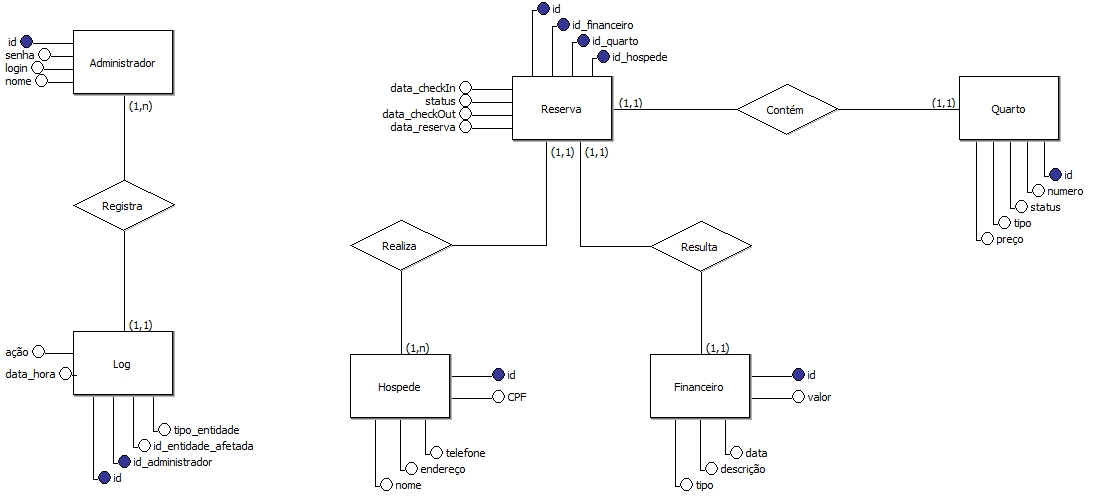
\includegraphics[width=\textwidth]{0406-MER.jpg}
	\caption{Modelo Entidade-Relacionamento (MER) desenvolvido no brModelo}
	\label{fig:mer}
\end{figure}
\subsection{Diagrama Entidade-Relacionamento - DER}
A Figura~\ref{fig:der} mostra o Diagrama Entidade-Relacionamento (DER) do sistema.

\begin{figure}[H]
	\centering
	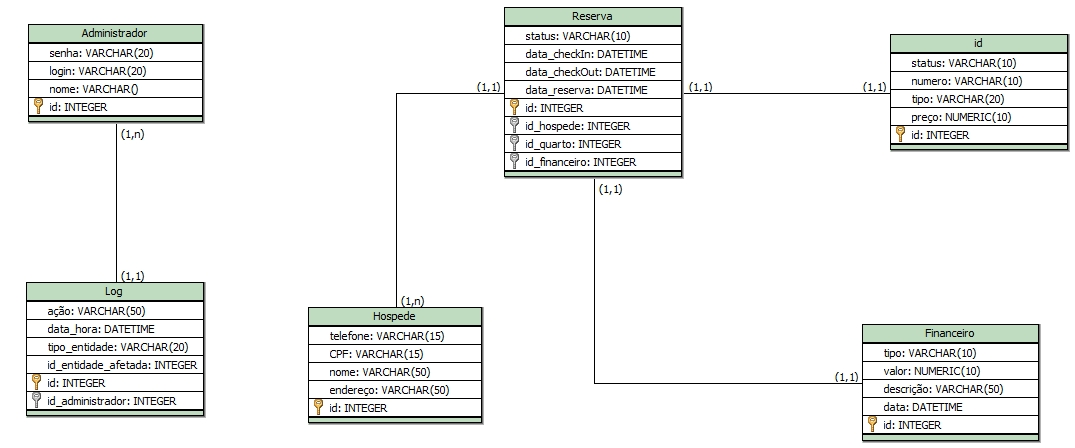
\includegraphics[width=\textwidth]{0406-DER.jpg}
	\caption{Diagrama Entidade-Relacionamento (MER) desenvolvido no brModelo}
	\label{fig:der}
\end{figure}


\section{Entregas}

\chapter{Viabilidade Financeira}
Visando a viabilidade financeira do desenvolvimento da aplicação de gestão de reservas de quarto, conduzimos um estudo dos custos necessários e produzimos relatórios referentes a diferentes cenários. Os dados utilizados no estudo são concretos e retirados de fontes seguras, nos ajudando a visualizar a factibilidade do projeto e ter melhor percepção para a tomada de decisões estratégicas.

\section{Custos}
\subsection{Custo Estrutural}

\begin{table}[h!]
	\centering
	\caption{Resumo dos custos de Equipamentos e Serviços}
	\label{tab:equipamentos-servicos}
	\begin{tabular}{|l|c|r|r|r|}
		\hline
		\textbf{Itens} & \textbf{Quantidade} & \textbf{Custo mensal} & \textbf{Total 4 meses} & \textbf{Total 9 meses} \\
		\hline
		Notebooks & 6 & R\$ 0,00 & R\$ 0,00 & R\$ 0,00 \\
		\hline
		Roteadores & 6 & R\$ 0,00 & R\$ 0,00 & R\$ 0,00 \\
		\hline
		Internet (Assinatura) & 6 & R\$ 114,97 & R\$ 2.759,28 & R\$ 6.208,38 \\
		\hline
		Eletricidade (Fatura) & 6 & R\$ 3,44 & R\$ 82,56 & R\$ 185,76 \\
		\hline
		\textbf{Total} & 24 & R\$ 118,41 & R\$ 2.841,84 & R\$ 6.394,14 \\
		\hline
	\end{tabular}
	\fonte{Elaborado pelos autores.}
\end{table}


\begin{table}[h!]
	\centering
	\caption{Resumo dos custos de Infraestrutura}
	\label{tab:infraestrutura}
	\begin{tabular}{|l|l|r|r|r|}
		\hline
		\textbf{Tipo} & \textbf{Serviço} & \textbf{Mensal} & \textbf{Total 4 meses} & \textbf{Total 9 meses} \\
		\hline
		Proxy Reverso & Servidor Nginx & R\$ 0,00 & R\$ 0,00 & R\$ 0,00 \\
		\hline
		Aplicação & Servidor Gunicorn & R\$ 0,00 & R\$ 0,00 & R\$ 0,00 \\
		\hline
		Framework Web & Servidor Django & R\$ 0,00 & R\$ 0,00 & R\$ 0,00 \\
		\hline
		Banco de Dados & PostgreSQL & R\$ 0,00 & R\$ 0,00 & R\$ 0,00 \\
		\hline
		Hospedagem & AWS & R\$ 0,00 & R\$ 0,00 & R\$ 0,00 \\
		\hline
		\textbf{Total} & & R\$ 0,00 & R\$ 0,00 & R\$ 0,00 \\
		\hline
	\end{tabular}
	\fonte{Elaborado pelos autores.}
\end{table}

\subsection{Custo Mão de Obra}

% Tabela 1 - Dados de horas
\begin{table}[H]
	\centering
	\caption{Quantidade e horas trabalhadas por função}
	\label{tab:mao-de-obra-horas}
	\adjustbox{max width=\textwidth}{
		\begin{tabular}{|>{\RaggedRight\arraybackslash}p{5.5cm}|c|c|c|c|}
			\hline
			\textbf{Função} & \textbf{Quantidade} & \textbf{Horas/Dia} & \textbf{Dias/Mês} & \textbf{Total de Horas/Mês} \\
			\hline
			Analista de Cronograma (PMO) & 1 & 6 & 22 & 25,90 \\
			\hline
			Engenheiro de Dados (DBA) & 1 & 6 & 22 & 47,30 \\
			\hline
			Analista de Documentação & 1 & 6 & 22 & 75,30 \\
			\hline
			Gerente de Projeto (PM) & 1 & 6 & 22 & 78,90 \\
			\hline
			Desenvolvedor Front-End & 1 & 6 & 22 & 150,00 \\
			\hline
			Desenvolvedor Back-End & 1 & 6 & 22 & 66,00 \\
			\hline
			\textbf{Total Mão de Obra} & 6 & 36 & 132 & 443,40 \\
			\hline
		\end{tabular}
	}
	\fonte{Elaborado pelos autores.}
\end{table}
\begin{table}[H]
	\centering
	\caption{Custos por função}
	\label{tab:mao-de-obra-custos}
	\adjustbox{max width=\textwidth}{
		\begin{tabular}{|>{\RaggedRight\arraybackslash}p{5.5cm}|r|r|r|r|}
			\hline
			\textbf{Função} & \textbf{Custo Hora (R\$)} & \textbf{Custo Mensal (R\$)} & \textbf{Total 4 meses (R\$)} & \textbf{Total 9 meses (R\$)} \\
			\hline
			Analista de Cronograma (PMO) & 16,00 & 155,40 & 621,60 & 1.398,60 \\
			\hline
			Engenheiro de Dados (DBA) & 13,00 & 283,80 & 1.135,20 & 2.554,20 \\
			\hline
			Analista de Documentação & 15,00 & 451,80 & 1.807,20 & 4.066,20 \\
			\hline
			Gerente de Projeto (PM) & 16,00 & 473,40 & 1.893,60 & 4.260,60 \\
			\hline
			Desenvolvedor Front-End & 13,00 & 900,00 & 3.600,00 & 8.100,00 \\
			\hline
			Desenvolvedor Back-End & 13,00 & 396,00 & 1.584,00 & 3.564,00 \\
			\hline
			\textbf{Total Mão de Obra} & 86,00 & 2.660,40 & 10.641,60 & 23.943,60 \\
			\hline
		\end{tabular}
	}
	\fonte{Elaborado pelos autores.}
\end{table}

\subsection{Custo Total}

\begin{table}[h!]
	\centering
	\caption{Custo Total por Categoria}
	\label{tab:custo-total}
	\adjustbox{max width=\textwidth}{
		\begin{tabular}{|l|r|r|r|}
			\hline
			\textbf{Categoria} & \textbf{Custo Mensal (R\$)} & \textbf{Custo Total (4 meses) (R\$)} & \textbf{Custo Total (9 meses) (R\$)} \\
			\hline
			Mão de Obra & 23.943,60 & 95.774,40 & 215.492,40 \\
			Estrutura & 118,41 & 473,64 & 1.065,69 \\
			\hline
			\textbf{Total} & 24.062,01 & 96.248,04 & 216.558,09 \\
			\hline
		\end{tabular}}
	\fonte{Elaborado pelos autores.}
\end{table}

\section{Cenários}

\subsection{Cenário Otimista}

\begin{figure}[H]
	\centering
	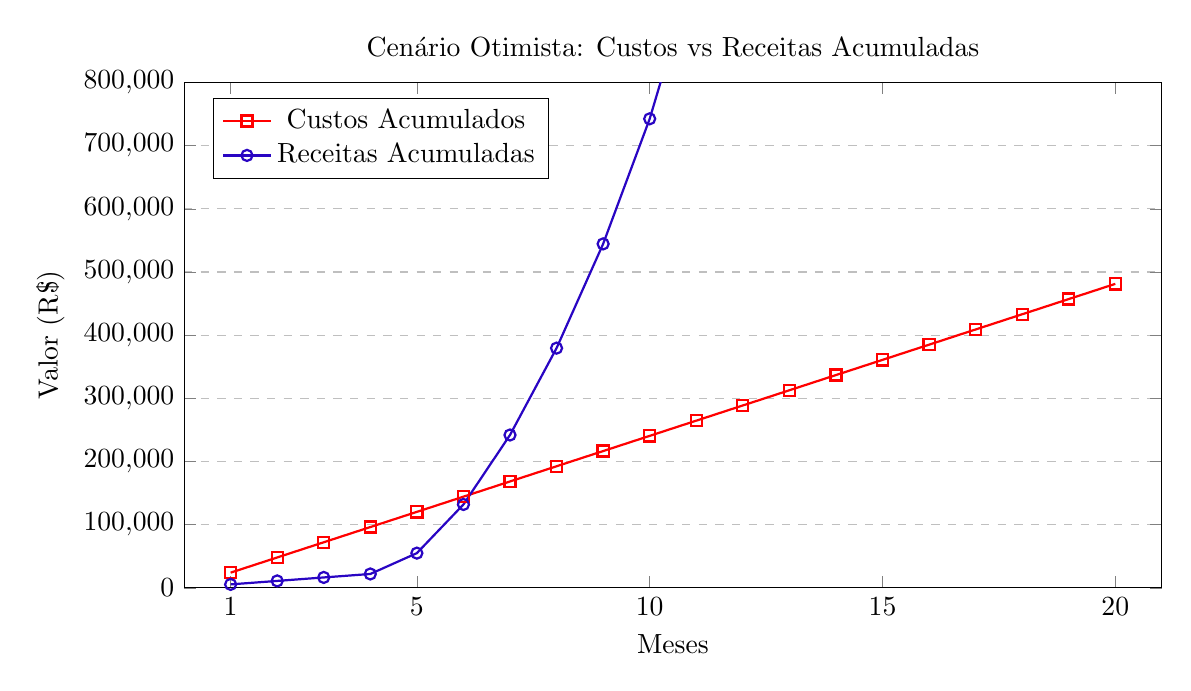
\begin{tikzpicture}
		\begin{axis}[
			title={Cenário Otimista: Custos vs Receitas Acumuladas},
			xlabel={Meses},
			ylabel={Valor (R\$)},
			xmin=0, xmax=21,
			ymin=0, ymax=800000,
			xtick={1,5,10,15,20},
			ytick={0,100000,200000,300000,400000,500000,600000,700000,800000},
			legend pos=north west,
			ymajorgrids=true,
			grid style=dashed,
			width=14cm,
			height=8cm,
			scaled y ticks = false,
			ticklabel style={/pgf/number format/fixed},
			]
			
			% Dados Custos Acumulados
			\addplot[
			color=red,
			mark=square,
			thick,
			]
			coordinates {
				(1,24062.01)
				(2,48124.02)
				(3,72186.03)
				(4,96248.04)
				(5,120310.05)
				(6,144372.06)
				(7,168434.07)
				(8,192496.08)
				(9,216558.09)
				(10,240620.10)
				(11,264682.11)
				(12,288744.12)
				(13,312806.13)
				(14,336868.14)
				(15,360930.15)
				(16,384992.16)
				(17,409054.17)
				(18,433116.18)
				(19,457178.19)
				(20,481240.20)
			};
			
			% Dados Receitas Acumuladas
			\addplot[
			color=blue,
			mark=o,
			thick,
			]
			coordinates {
				(1,5500)
				(2,11000)
				(3,16500)
				(4,22000)
				(5,55000)
				(6,132000)
				(7,242000)
				(8,379500)
				(9,544500)
				(10,742500)
				(11,990000)
				(12,1276000)
				(13,1606000)
				(14,1991000)
				(15,2431000)
				(16,2926000)
				(17,3476000)
				(18,4108500)
				(19,4823500)
				(20,5577000)
			};
			
			\legend{Custos Acumulados, Receitas Acumuladas}
		\end{axis}
	\end{tikzpicture}
	\caption{Comparação dos custos e receitas acumuladas no cenário otimista}
	\label{fig:custo-receita}
\end{figure}



\subsection{Cenário Pessimista}


\begin{figure}[H]
	\centering
	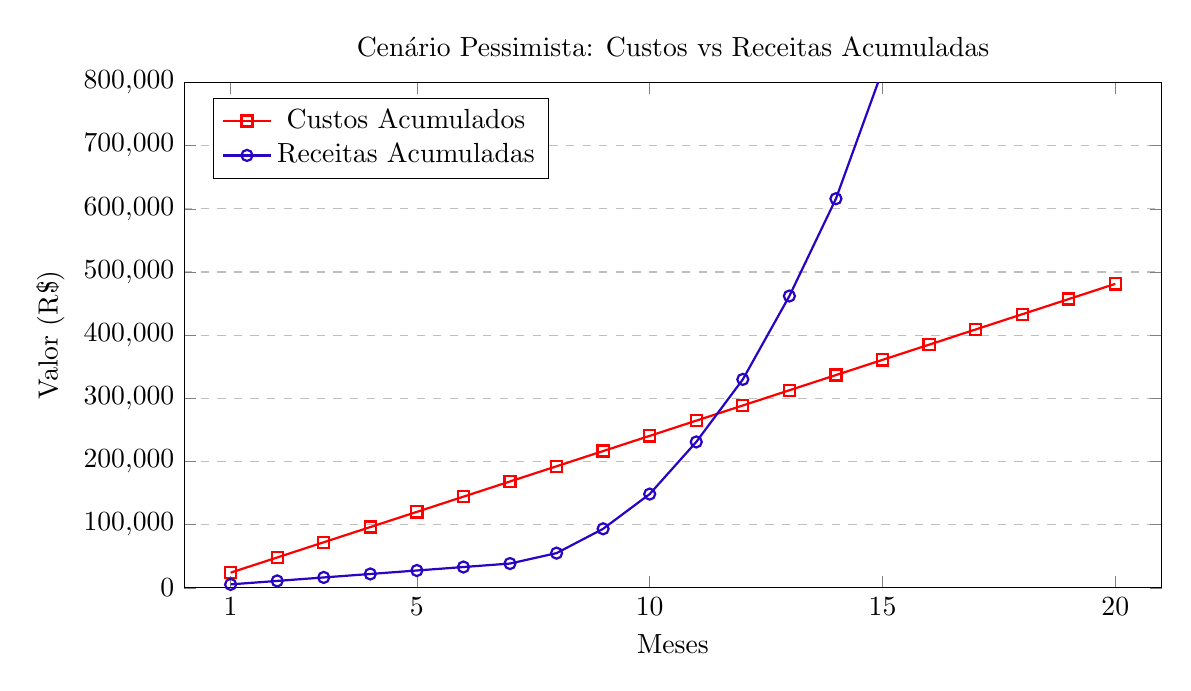
\begin{tikzpicture}
		\begin{axis}[
			title={Cenário Pessimista: Custos vs Receitas Acumuladas},
			xlabel={Meses},
			ylabel={Valor (R\$)},
			xmin=0, xmax=21,
			ymin=0, ymax=800000,
			xtick={1,5,10,15,20},
			ytick={0,100000,200000,300000,400000,500000,600000,700000,800000},
			legend pos=north west,
			ymajorgrids=true,
			grid style=dashed,
			width=14cm,
			height=8cm,
			scaled y ticks = false,
			ticklabel style={/pgf/number format/fixed},
			]
			
			% Dados Custos Acumulados
			\addplot[
			color=red,
			mark=square,
			thick,
			]
			coordinates {
				(1,24062.01)
				(2,48124.02)
				(3,72186.03)
				(4,96248.04)
				(5,120310.05)
				(6,144372.06)
				(7,168434.07)
				(8,192496.08)
				(9,216558.09)
				(10,240620.10)
				(11,264682.11)
				(12,288744.12)
				(13,312806.13)
				(14,336868.14)
				(15,360930.15)
				(16,384992.16)
				(17,409054.17)
				(18,433116.18)
				(19,457178.19)
				(20,481240.20)
			};
			
			% Dados Receitas Acumuladas (soma acumulada)
			\addplot[
			color=blue,
			mark=o,
			thick,
			]
			coordinates {
				(1,5500)
				(2,11000)
				(3,16500)
				(4,22000)
				(5,27500)
				(6,33000)
				(7,38500)
				(8,55000)
				(9,93500)
				(10,148500)
				(11,231000)
				(12,330000)
				(13,462000)
				(14,616000)
				(15,819500)
				(16,1078000)
				(17,1397000)
				(18,1809500)
				(19,2304500)
				(20,2876500)
			};
			
			\legend{Custos Acumulados, Receitas Acumuladas}
		\end{axis}
	\end{tikzpicture}
	\caption{Comparação dos custos e receitas acumuladas no cenário pessimista}
	\label{fig:custo-receita-pessimista}
\end{figure}



\subsection{Cenário Realista}


\begin{figure}[H]
	\centering
	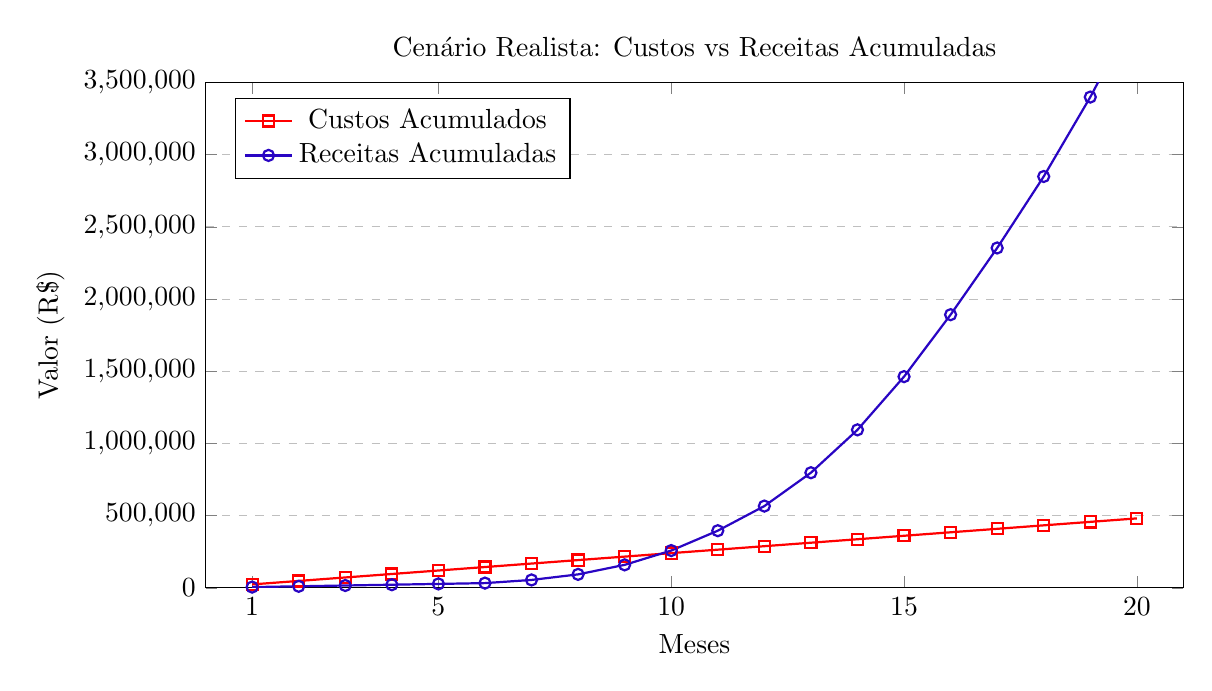
\begin{tikzpicture}
		\begin{axis}[
			title={Cenário Realista: Custos vs Receitas Acumuladas},
			xlabel={Meses},
			ylabel={Valor (R\$)},
			xmin=0, xmax=21,
			ymin=0, ymax=3500000,
			xtick={1,5,10,15,20},
			ytick={0,500000,1000000,1500000,2000000,2500000,3000000,3500000},
			legend pos=north west,
			ymajorgrids=true,
			grid style=dashed,
			width=14cm,
			height=8cm,
			scaled y ticks=false,
			ticklabel style={/pgf/number format/fixed},
			]
			
			% Dados Custos Acumulados
			\addplot[
			color=red,
			mark=square,
			thick,
			]
			coordinates {
				(1,24062.01)
				(2,48124.02)
				(3,72186.03)
				(4,96248.04)
				(5,120310.05)
				(6,144372.06)
				(7,168434.07)
				(8,192496.08)
				(9,216558.09)
				(10,240620.10)
				(11,264682.11)
				(12,288744.12)
				(13,312806.13)
				(14,336868.14)
				(15,360930.15)
				(16,384992.16)
				(17,409054.17)
				(18,433116.18)
				(19,457178.19)
				(20,481240.20)
			};
			
			% Dados Receitas Acumuladas (soma acumulada)
			\addplot[
			color=blue,
			mark=o,
			thick,
			]
			coordinates {
				(1,5500)
				(2,11000)
				(3,16500)
				(4,22000)
				(5,27500)
				(6,33000)
				(7,55000)
				(8,93500)
				(9,159500)
				(10,258500)
				(11,396000)
				(12,566500)
				(13,797500)
				(14,1094500)
				(15,1463000)
				(16,1892000)
				(17,2354000)
				(18,2849000)
				(19,3399000)
				(20,4009500)
			};
			
			\legend{Custos Acumulados, Receitas Acumuladas}
		\end{axis}
	\end{tikzpicture}
	\caption{Comparação dos custos e receitas acumuladas no cenário realista}
	\label{fig:custo-receita-realista}
\end{figure}



\chapter{Considerações Finais}

%
% ----------------------------------------------------------
% Finaliza a parte no bookmark do PDF
% para que se inicie o bookmark na raiz
% e adiciona espaço de parte no Sumário
% ----------------------------------------------------------
\phantompart

% ---
% Conclusão
% ---
\chapter{Conclusão}
% ---

\lipsum[31-33]

% ----------------------------------------------------------
% ELEMENTOS PÓS-TEXTUAIS
% ----------------------------------------------------------
\postextual
% ----------------------------------------------------------

% ----------------------------------------------------------
% Referências bibliográficas
% ----------------------------------------------------------
\bibliography{abntex2-modelo-references}

% ----------------------------------------------------------
% Glossário
% ----------------------------------------------------------
%
% Consulte o manual da classe abntex2 para orientações sobre o glossário.
%
%\glossary

% ----------------------------------------------------------
% Apêndices
% ----------------------------------------------------------

% ---
% Inicia os apêndices
% ---
\begin{apendicesenv}

% Imprime uma página indicando o início dos apêndices
\partapendices

% ----------------------------------------------------------
\chapter{Quisque libero justo}
% ----------------------------------------------------------

\lipsum[50]

% ----------------------------------------------------------
\chapter{Nullam elementum urna vel imperdiet sodales elit ipsum pharetra ligula
ac pretium ante justo a nulla curabitur tristique arcu eu metus}
% ----------------------------------------------------------
\lipsum[55-57]

\end{apendicesenv}
% ---


% ----------------------------------------------------------
% Anexos
% ----------------------------------------------------------

% ---
% Inicia os anexos
% ---
\begin{anexosenv}

% Imprime uma página indicando o início dos anexos
\partanexos

% ---
\chapter{Morbi ultrices rutrum lorem.}
% ---
\lipsum[30]

% ---
\chapter{Cras non urna sed feugiat cum sociis natoque penatibus et magnis dis
parturient montes nascetur ridiculus mus}
% ---

\lipsum[31]

% ---
\chapter{Fusce facilisis lacinia dui}
% ---

\lipsum[32]

\end{anexosenv}

%---------------------------------------------------------------------
% INDICE REMISSIVO
%---------------------------------------------------------------------
\phantompart
\printindex
%---------------------------------------------------------------------

\end{document}
